\documentclass{beamer}


%%%%% 26-02-2022 package multicol multirow
\newcommand{\mc}[2]{\multicolumn{#1}{c}{#2}}
\definecolor{Gray}{gray}{0.85}
\definecolor{LightCyan}{rgb}{0.88,1,1}
\usepackage{hhline,longtable}
\usepackage{tabularx,booktabs}

\usepackage{multicol}
\usepackage{multirow}
%% 26-02-2022
\usepackage{hhline,longtable}
\usepackage{threeparttable}

\usepackage{tabularx,booktabs}
\newcommand{\tabitem}{~~\llap{\textbullet}~~}


\usepackage{enumerate}
\usepackage[shortlabels]{enumitem}

\setlist[enumerate, 1]{label =\textbf{\arabic*.}}
\setlist[enumerate, 2]{label =\textbf{\theenumi \alph*}}
\usepackage{array,multirow}

\usepackage{amsmath,mathtools}

\usepackage{amssymb}
\usepackage{amsthm}
\usepackage{mathtools}



\DeclarePairedDelimiter\abs{\lvert}{\rvert}%
\DeclarePairedDelimiter\norm{\lVert}{\rVert}%

% Swap the definition of \abs* and \norm*, so that \abs
% and \norm resizes the size of the brackets, and the 
% starred version does not.
\makeatletter
\let\oldabs\abs
\def\abs{\@ifstar{\oldabs}{\oldabs*}}










%%%% animation package 21-09-2021
\usepackage{animate}


%%%%%%%%%%%%%%%%%09-09-2021\\\ copied from Webinarinnovation page
% Here I would like to make a new command to change the transparency of a photo and put it as a background photo
\usepackage{tikz}



%%%%%%%%%%%% 22-10-2020 Background block package
% beamer: How to place images behind text (z-order)
% (http://tex.stackexchange.com/a/134311)
\makeatletter
\newbox\@backgroundblock
\newenvironment{backgroundblock}[2]{%
  \global\setbox\@backgroundblock=\vbox\bgroup%
    \unvbox\@backgroundblock%
    \vbox to0pt\bgroup\vskip#2\hbox to0pt\bgroup\hskip#1\relax%
}{\egroup\egroup\egroup}
\addtobeamertemplate{background}{\box\@backgroundblock}{}
\makeatother

%%%%%%%%%%%%%%%%%%%%%%%%%%%%%%%%%%%%%%%%%%%%
%%%%%%%%%%%26-10-2020% set figure number
\setbeamertemplate{caption}[numbered]


%%%%%%%%%%%%%%%%26-10-2020
\usepackage{amssymb,amsmath}


%%%%%%%%%%%%%%%%26-10-2020
\newenvironment{variableblock}[3]{%
  \setbeamercolor{block body}{#2}
  \setbeamercolor{block title}{#3}
  \begin{block}{#1}}{\end{block}}
  
  \setbeamercolor{block body alerted}{bg=alerted text.fg!10}
\setbeamercolor{block title alerted}{bg=alerted text.fg!20}
\setbeamercolor{block body}{bg=structure!10}
\setbeamercolor{block title}{bg=structure!20}
\setbeamercolor{block body example}{bg=green!10}
\setbeamercolor{block title example}{bg=green!20}

\setbeamertemplate{blocks}[rounded][shadow=true]


%%%%%%%%%%%%%%%%%%%%%26-10-2020
\setbeamertemplate{footline}[frame number]

%%%%%%%%%%%% 26-10-2020
\usepackage{color, colortbl}
\definecolor{Gray}{gray}{0.85}

%%%%%%%%%%%%%%%%%%27-10-2020
\usepackage[T1]{fontenc}



\title{\large \textbf{Large-Scale Integration of EVs, one Application of the High-Performace Solver: BATTPOWER}}
\begin{backgroundblock}{20mm}{20mm}
    \begin{tikzpicture}
    \node[anchor=east,inner sep=0] (B) at (4,0) {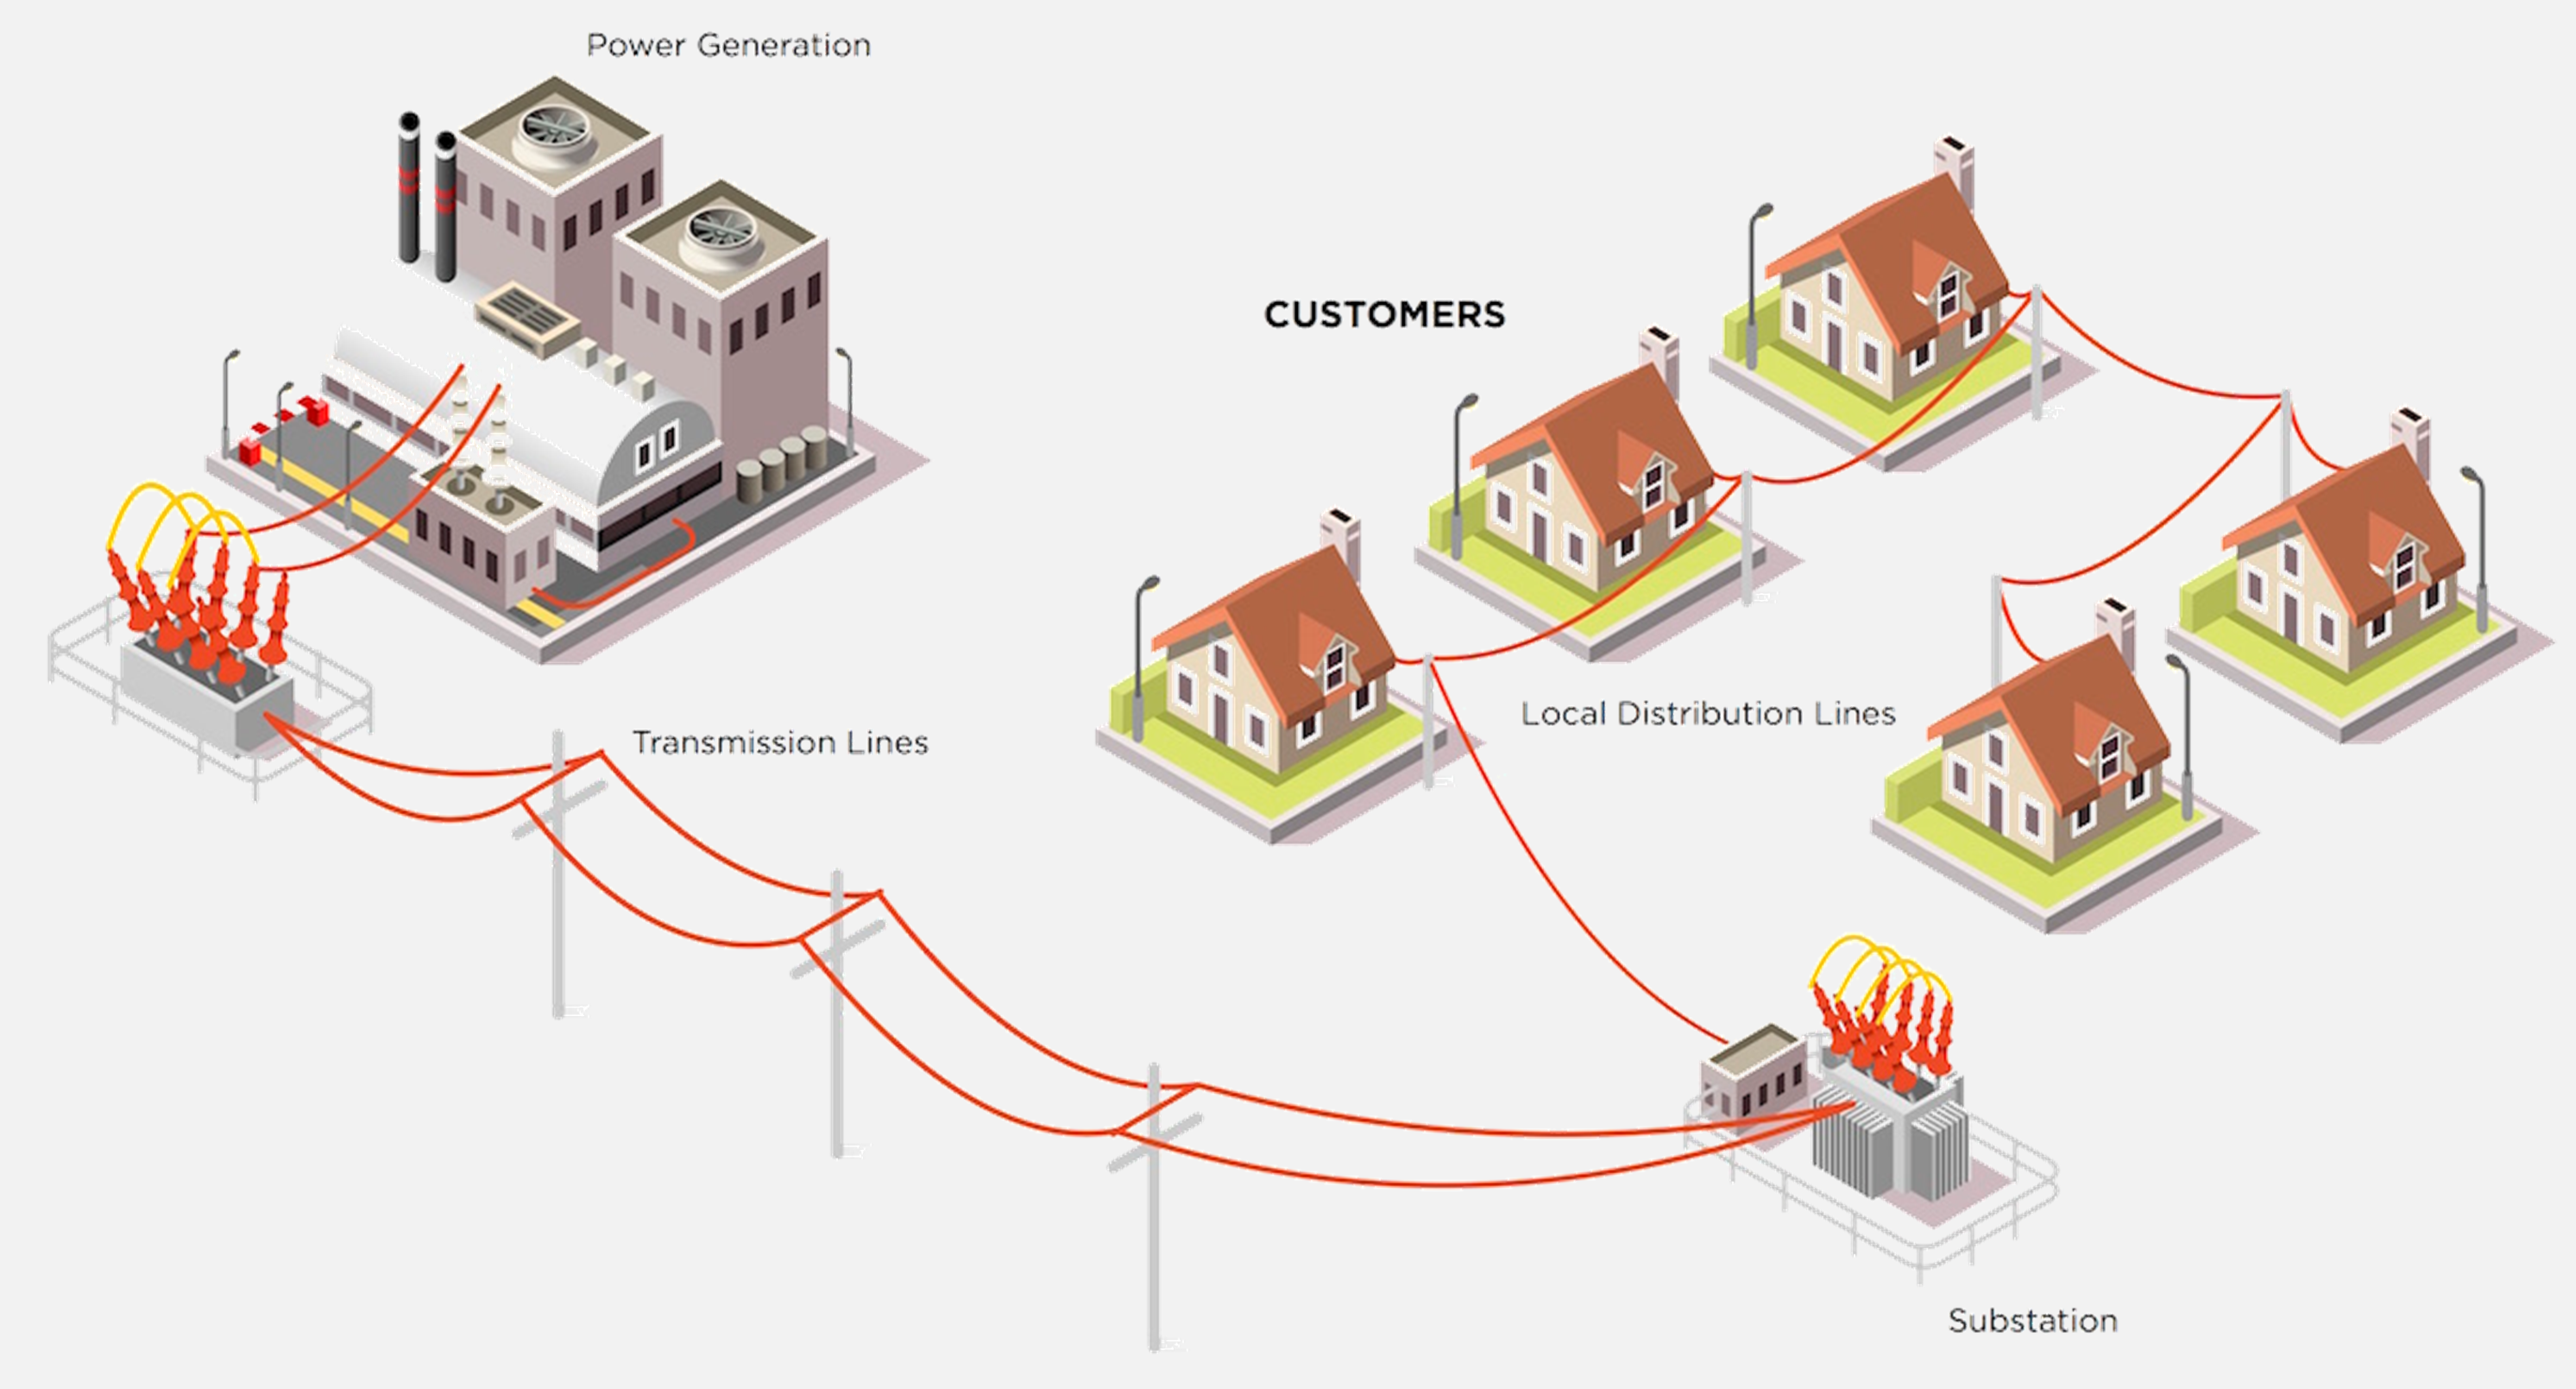
\includegraphics[width=\linewidth]{Figures/PowerSys.png}};
           \fill [draw=none, fill=white, fill opacity=0.7] (B.north west) -- (B.north east) -- (B.south east) -- (B.south west) -- (B.north west) -- cycle;
 
    \end{tikzpicture} 
    \end{backgroundblock} 

\logo{%
    
\includegraphics[width=3cm,height=3cm,keepaspectratio]{ntnulogo_eng}~%
}


\author{Salman Zaferanlouei}
\institute{NTNU{\\ \vskip 1cm} \scalebox{1.5}{\insertlogo}}
\date{\today}









\begin{document}
\begin{frame}
\titlepage
\end{frame}
%%%%%%%%%%%%%%%%%%%%%%%%%%%%%%%%%%%%%%%%%%
%%%%%%%%%%%%%%%%%%%%%%%%%%%%%%%%%%%%%%%%%%
%%%%%%%%%%%%%%%%%%%%%%%%%%%%%%%%%%%%%%%%%%
%%%%%%%%%%%%%%%%%%%%%%%%%%%%%%%%%%%%%%%%%%
\begin{frame}{The answer is yes}

\begin{table}
\small
\def\firstrowcolor{}
\def\secondrowcolor{}
\onslide<1->{\def\firstrowcolor{\rowcolor{Gray}}}
\caption{Charge Scheduling Strategies}
\label{tab:termination}
\begin{tabular}{l c c} 
\hline
 \firstrowcolor Method &  \begin{tabular}[c]{@{}c@{}}Max EV\\ hosting Capacity\end{tabular}&  \\  
  Uncoordinated/Dumb Charging& 20\%& 
\includegraphics[width=.1\textwidth]{Figures/RedMark.png} \\
 \onslide<1->{Market price based &  36\%& 
\includegraphics[width=.1\textwidth]{Figures/YellowMark.png}} \\
 \onslide<1->{\begin{tabular}[c]{@{}l@{}}Market price and\\ Congestion management based\end{tabular}& 100\%& 
\includegraphics[width=.1\textwidth]{Figures/GreenMark.png} }\\
\hline
\end{tabular}
\end{table}
\end{frame}
%%%%%%%%%%%%%%%%%%%%%%%%%%%%%%%%%%%%%%%%%%
%%%%%%%%%%%%%%%%%%%%%%%%%%%%%%%%%%%%%%%%%%
%%%%%%%%%%%%%%%%%%%%%%%%%%%%%%%%%%%%%%%%%%
%%%%%%%%%%%%%%%%%%%%%%%%%%%%%%%%%%%%%%%%%%

\section{Purpose/Content}
\begin{frame}{The presentation goal}
\begin{itemize}
\item \textbf{Purpose:} To show how to coordinate \textcolor{red}{\textbf{Batteries in the Grid: (EVs):}} Large-Scale EV charge scheduling platform to avoid congestion 
\item \textbf{Phase I:} Background and Motivation
\item \textbf{Phase II:} EV Statistics
\item \textbf{Phase III:} Case Study
\end{itemize}
\begin{center}
\begin{tabular}{|l l|} 
\hline
\rowcolor{Gray} \textbf{Project Name:} &BATTPOWER \\
\textbf{Presentation Time:}& 10 min \\
\hline
\end{tabular}
\end{center}
\end{frame}

%%%%%%%%%%%%%%%%%%%%%%%%%%%%%%%%%%%%%%%%%%
%%%%%%%%%%%%%%%%%%%%%%%%%%%%%%%%%%%%%%%%%%
%%%%%%%%%%%%%%%%%%%%%%%%%%%%%%%%%%%%%%%%%%
%%%%%%%%%%%%%%%%%%%%%%%%%%%%%%%%%%%%%%%%%%
%%%%%%%%%%%%%%%%%%%%%%%%%%%%%%%%%%%%%%%%%%
%%%%%%%%%%%%%%%%%%%%%%%%%%%%%%%%%%%%%
%%%%%%%%%%%%%%%%%%%%%%%%%%%%%%%%%%%%%%%%%%
%%%%%%%%%%%%%%%%%%%%%%%%%%%%%%%%%%%%%%%%%%
%%%%%%%%%%%%%%%%%%%%%%%%%%%%%%%%%%%%%%%%%%
%%%%%%%%%%%%%%%%%%%%%%%%%%%%%%%%%%%%%%%%%%
\begin{frame}[plain]
\begin{tikzpicture}[overlay, remember picture]
\node[anchor=center] at (current page.center) {
\begin{beamercolorbox}[center]{title}
     Phase I:\\\textbf{Background and Motivation}
  \end{beamercolorbox}};
\end{tikzpicture}

\end{frame}
%%%%%%%%%%%%%%%%%%%%%%%%%%%%%%%%%%%%%%%%%%
%%%%%%%%%%%%%%%%%%%%%%%%%%%%%%%%%%%%%%%%%%
%%%%%%%%%%%%%%%%%%%%%%%%%%%%%%%%%%%%%%%%%%
%%%%%%%%%%%%%%%%%%%%%%%%%%%%%%%%%%%%%%%%%%
\section{Background}
\begin{frame}{Electricity Grid}
\begin{figure}[!htbp]
\centering
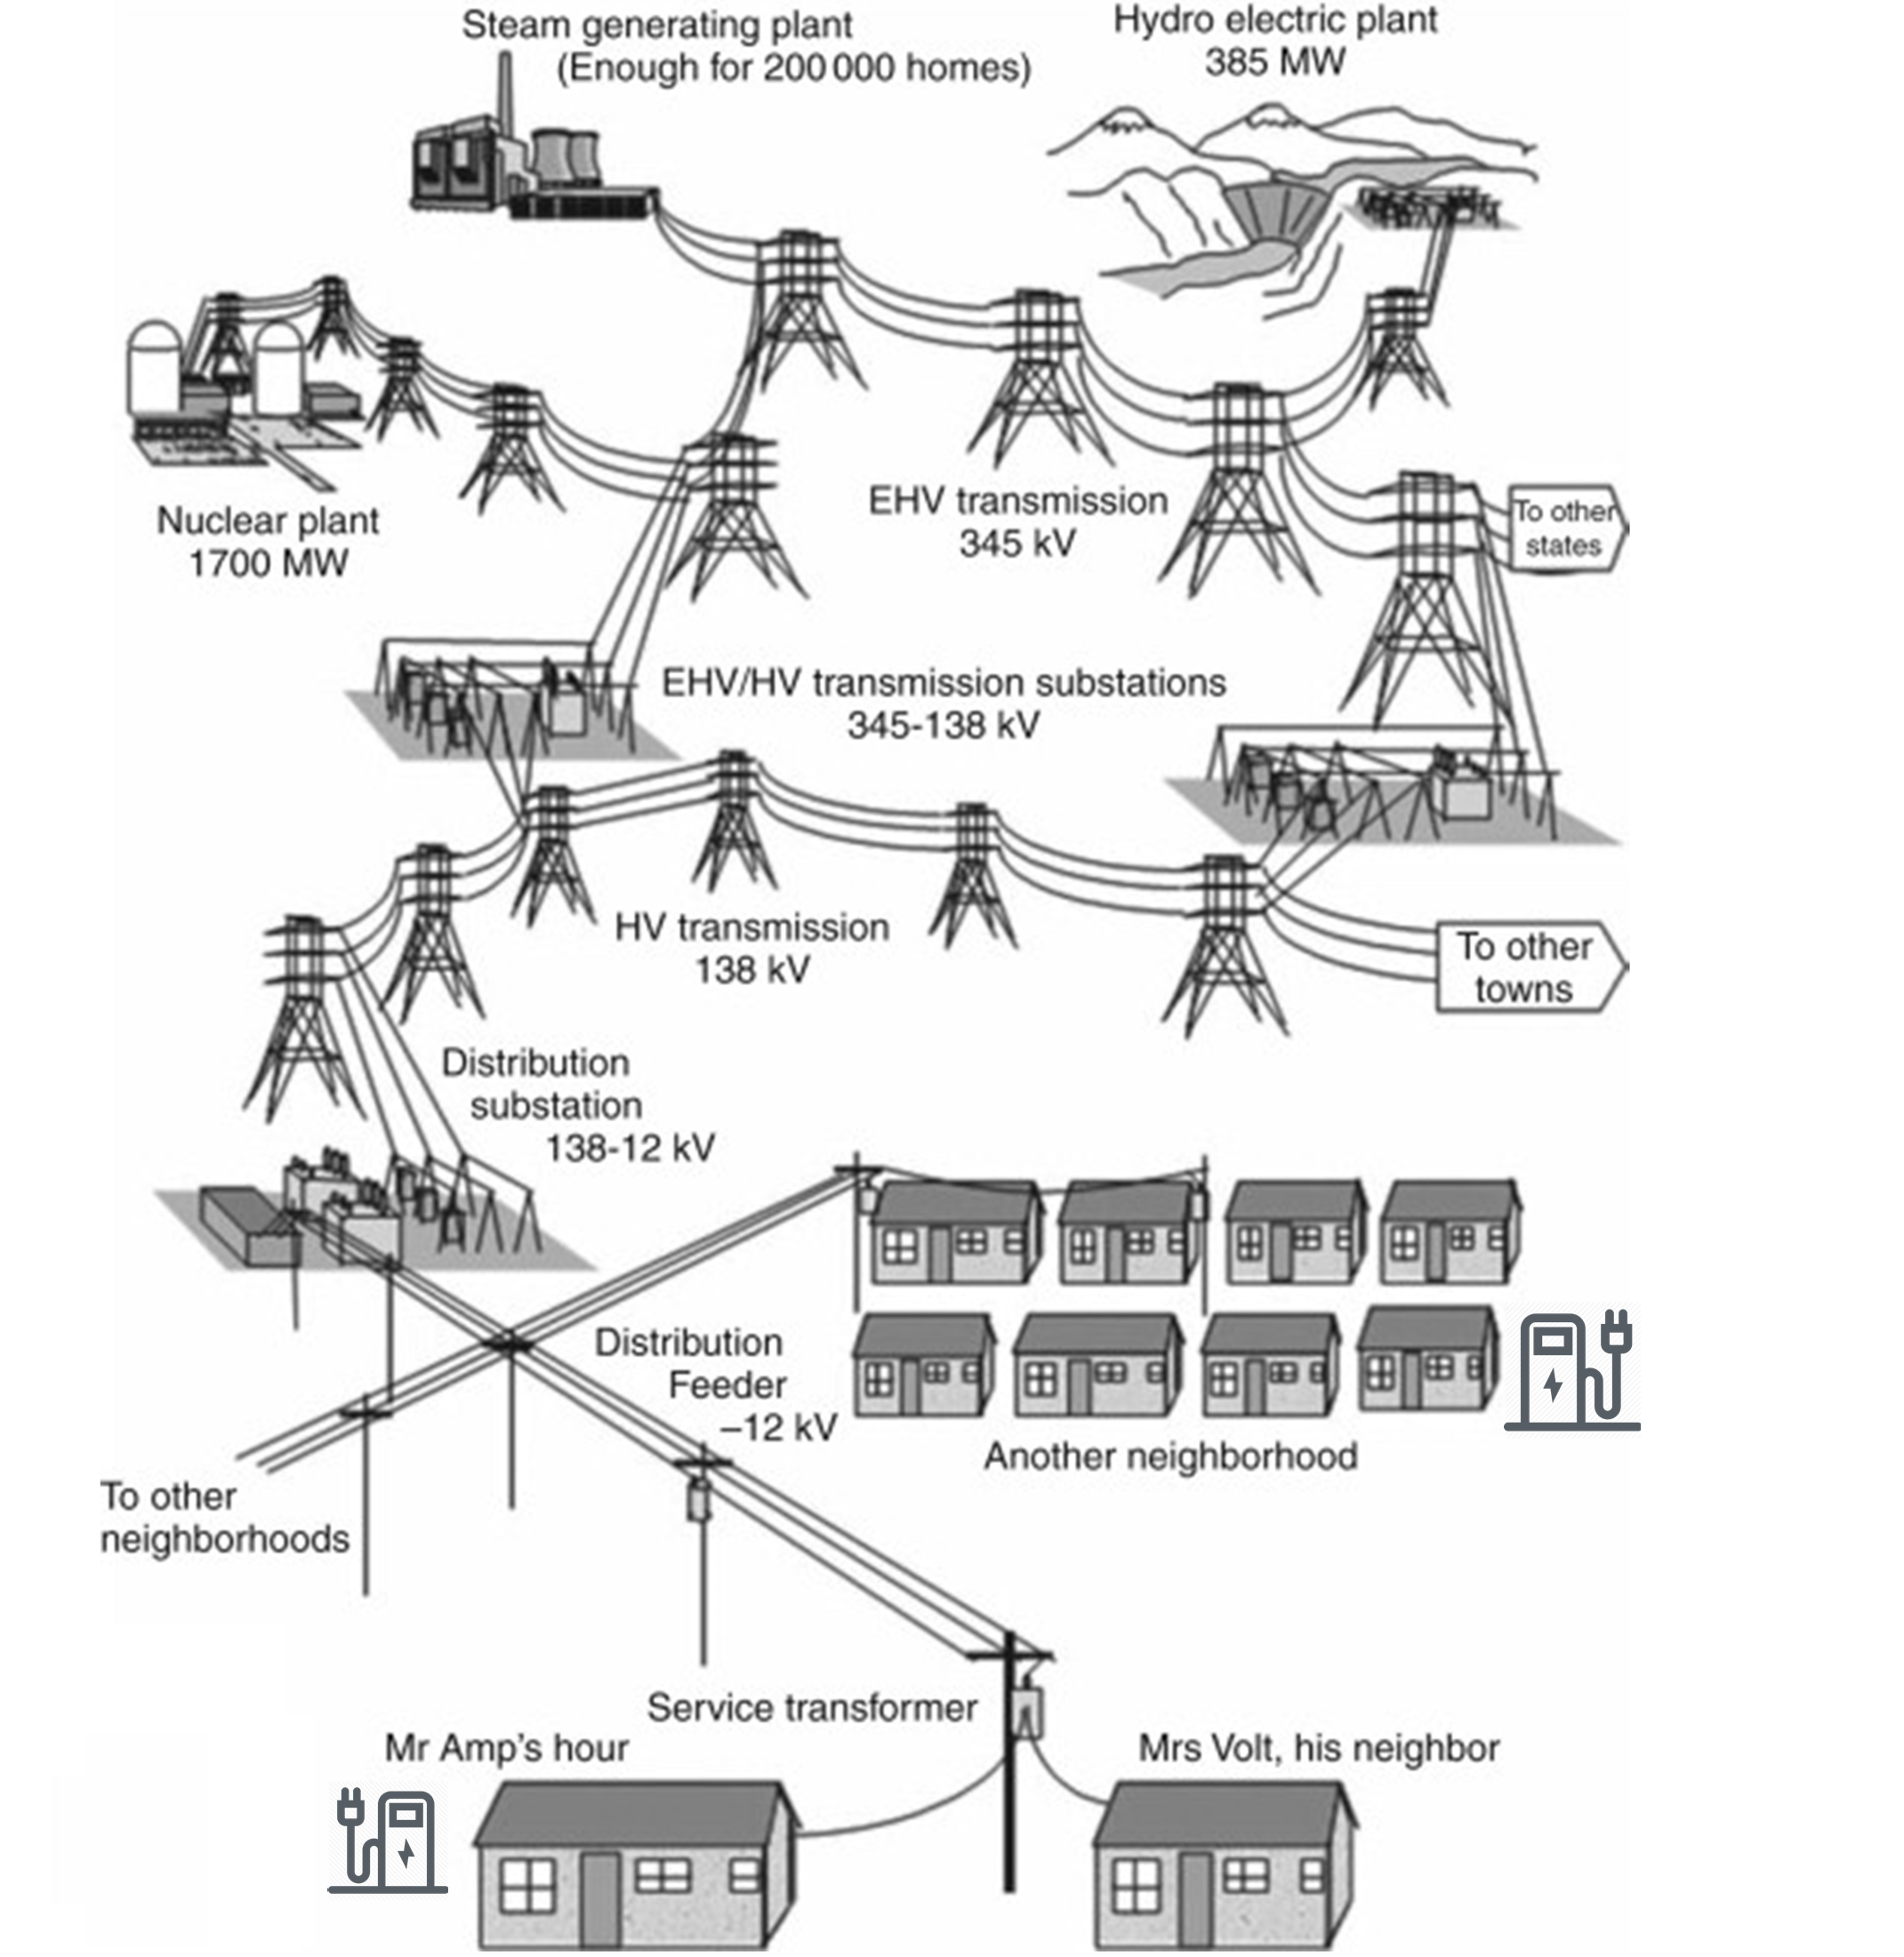
\includegraphics[width=2.8 in , height=2.4 in]{Figures/EVchalendge1.png}
\caption{\tiny[www.sciencedirect.com/science/article/pii/B9781845697846500019]}
\end{figure}
\end{frame}





%%%%%%%%%%%%%%%%%%%%%%%%%%%%%%%%%%%%%%%%%%
%%%%%%%%%%%%%%%%%%%%%%%%%%%%%%%%%%%%%%%%%%
%%%%%%%%%%%%%%%%%%%%%%%%%%%%%%%%%%%%%%%%%%
%%%%%%%%%%%%%%%%%%%%%%%%%%%%%%%%%%%%%%%%%%

\begin{frame}{Sustainability/Green shift/CO\textsubscript{2} reduction}
\begin{alertblock}{\textcolor{red}{For many reasons power electricity grid is facing decentralization}}
\begin{itemize}
\item<1-> Phasing out coal (carbon-heavy sources of production) and nuclear power plants
\item<2-> Increase penetration of solar and wind production
\end{itemize}
\end{alertblock}
\begin{columns}
    \column{0.5\textwidth}
    This chain between large power producers and consumers is weakened.
    \column{0.5\textwidth}
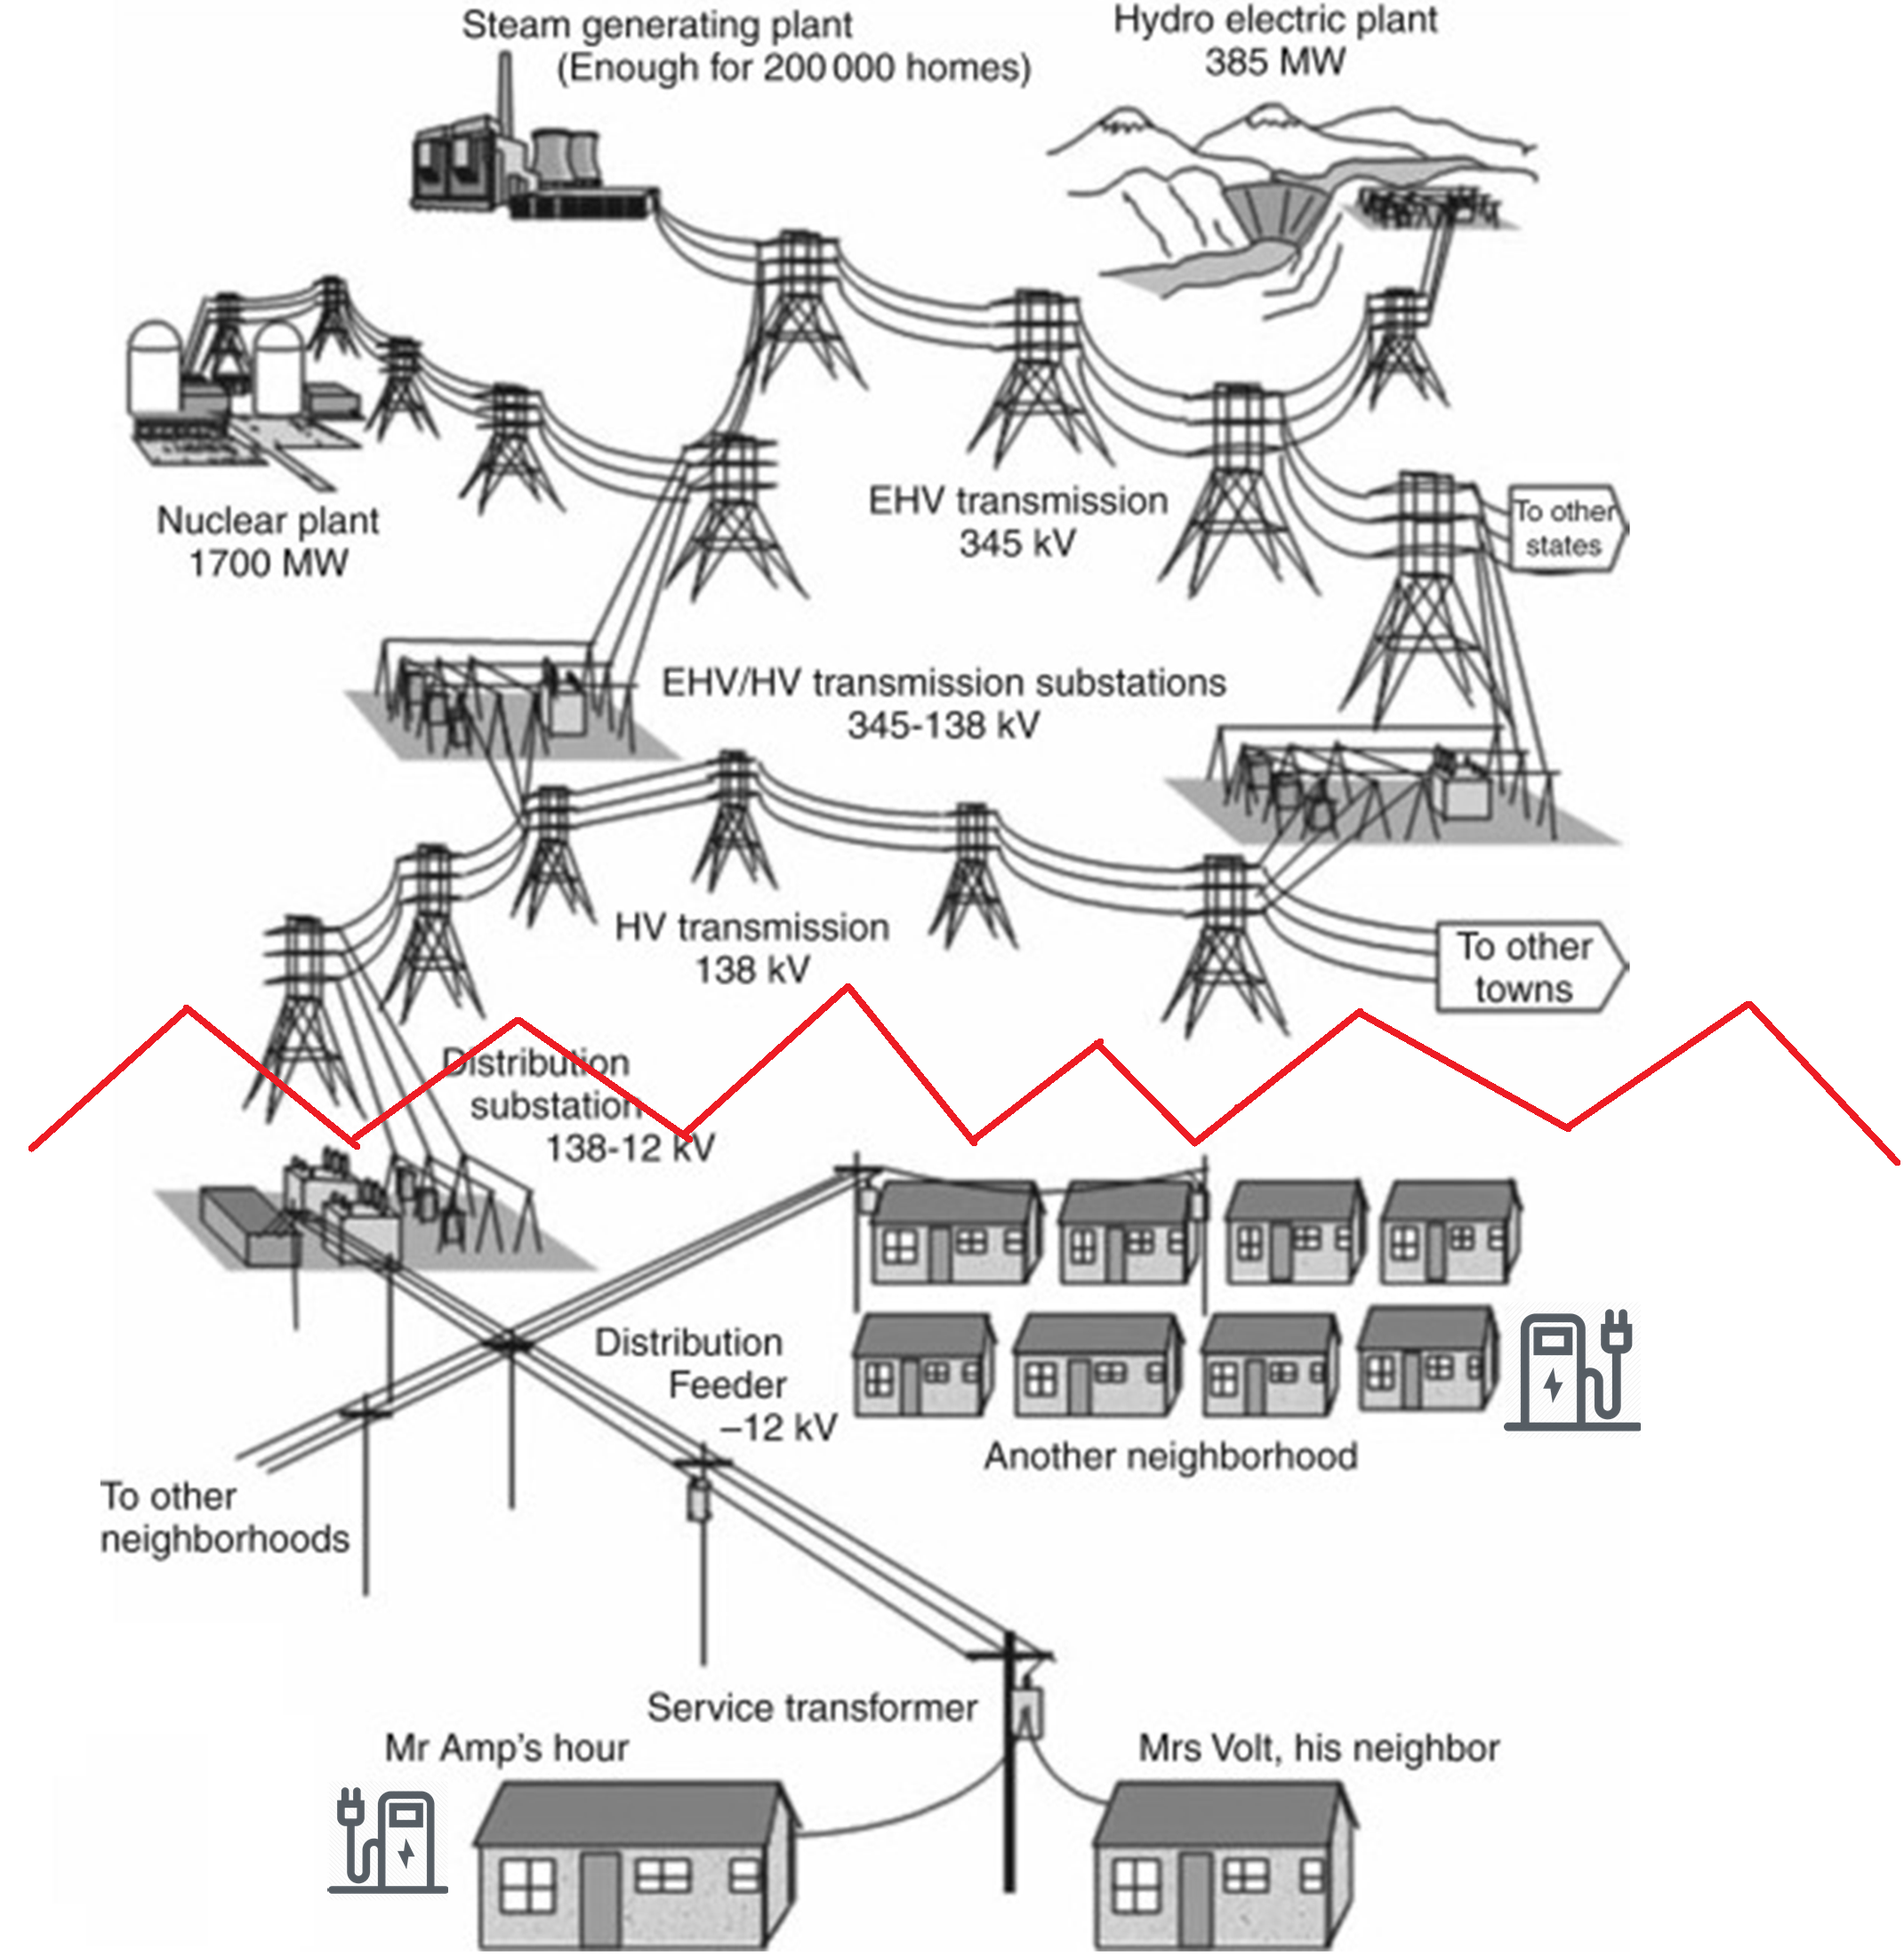
\includegraphics[width=2 in , height=1.6 in]{Figures/EVchalendgebreak.png}
\end{columns}
\end{frame}



\section{Background}
\begin{frame}{Background: cont.}
\begin{block}{Items}
\begin{itemize}
\item <1-> \small Green shift in electricity systems is needed for the reduction of $\mathrm{CO_2}$ emissions
\begin{itemize}
\item<2-> \tiny  Integration of Distributed Energy Resources (DER) is a huge challenge
\end{itemize}
\only<2>{ \begin{alertblock}{\tiny Note}
{\tiny DER includes Renewable Energy, Energy Storage, Electric Vehicles and Flexible Demand}
\end{alertblock}}
\item<3->\small Grid companies must be able to analyse the impacts of DER 
\only<4>{ \begin{alertblock}{Note}
\textbf{\tiny Optimal Power Flow (OPF)}{\tiny solvers are essential}
\end{alertblock}}
\item<5->\small The inegration of DER in smart grids calls for \textbf{much more sophisticated solvers} for OPF
\end{itemize}
\end{block}
\begin{figure}
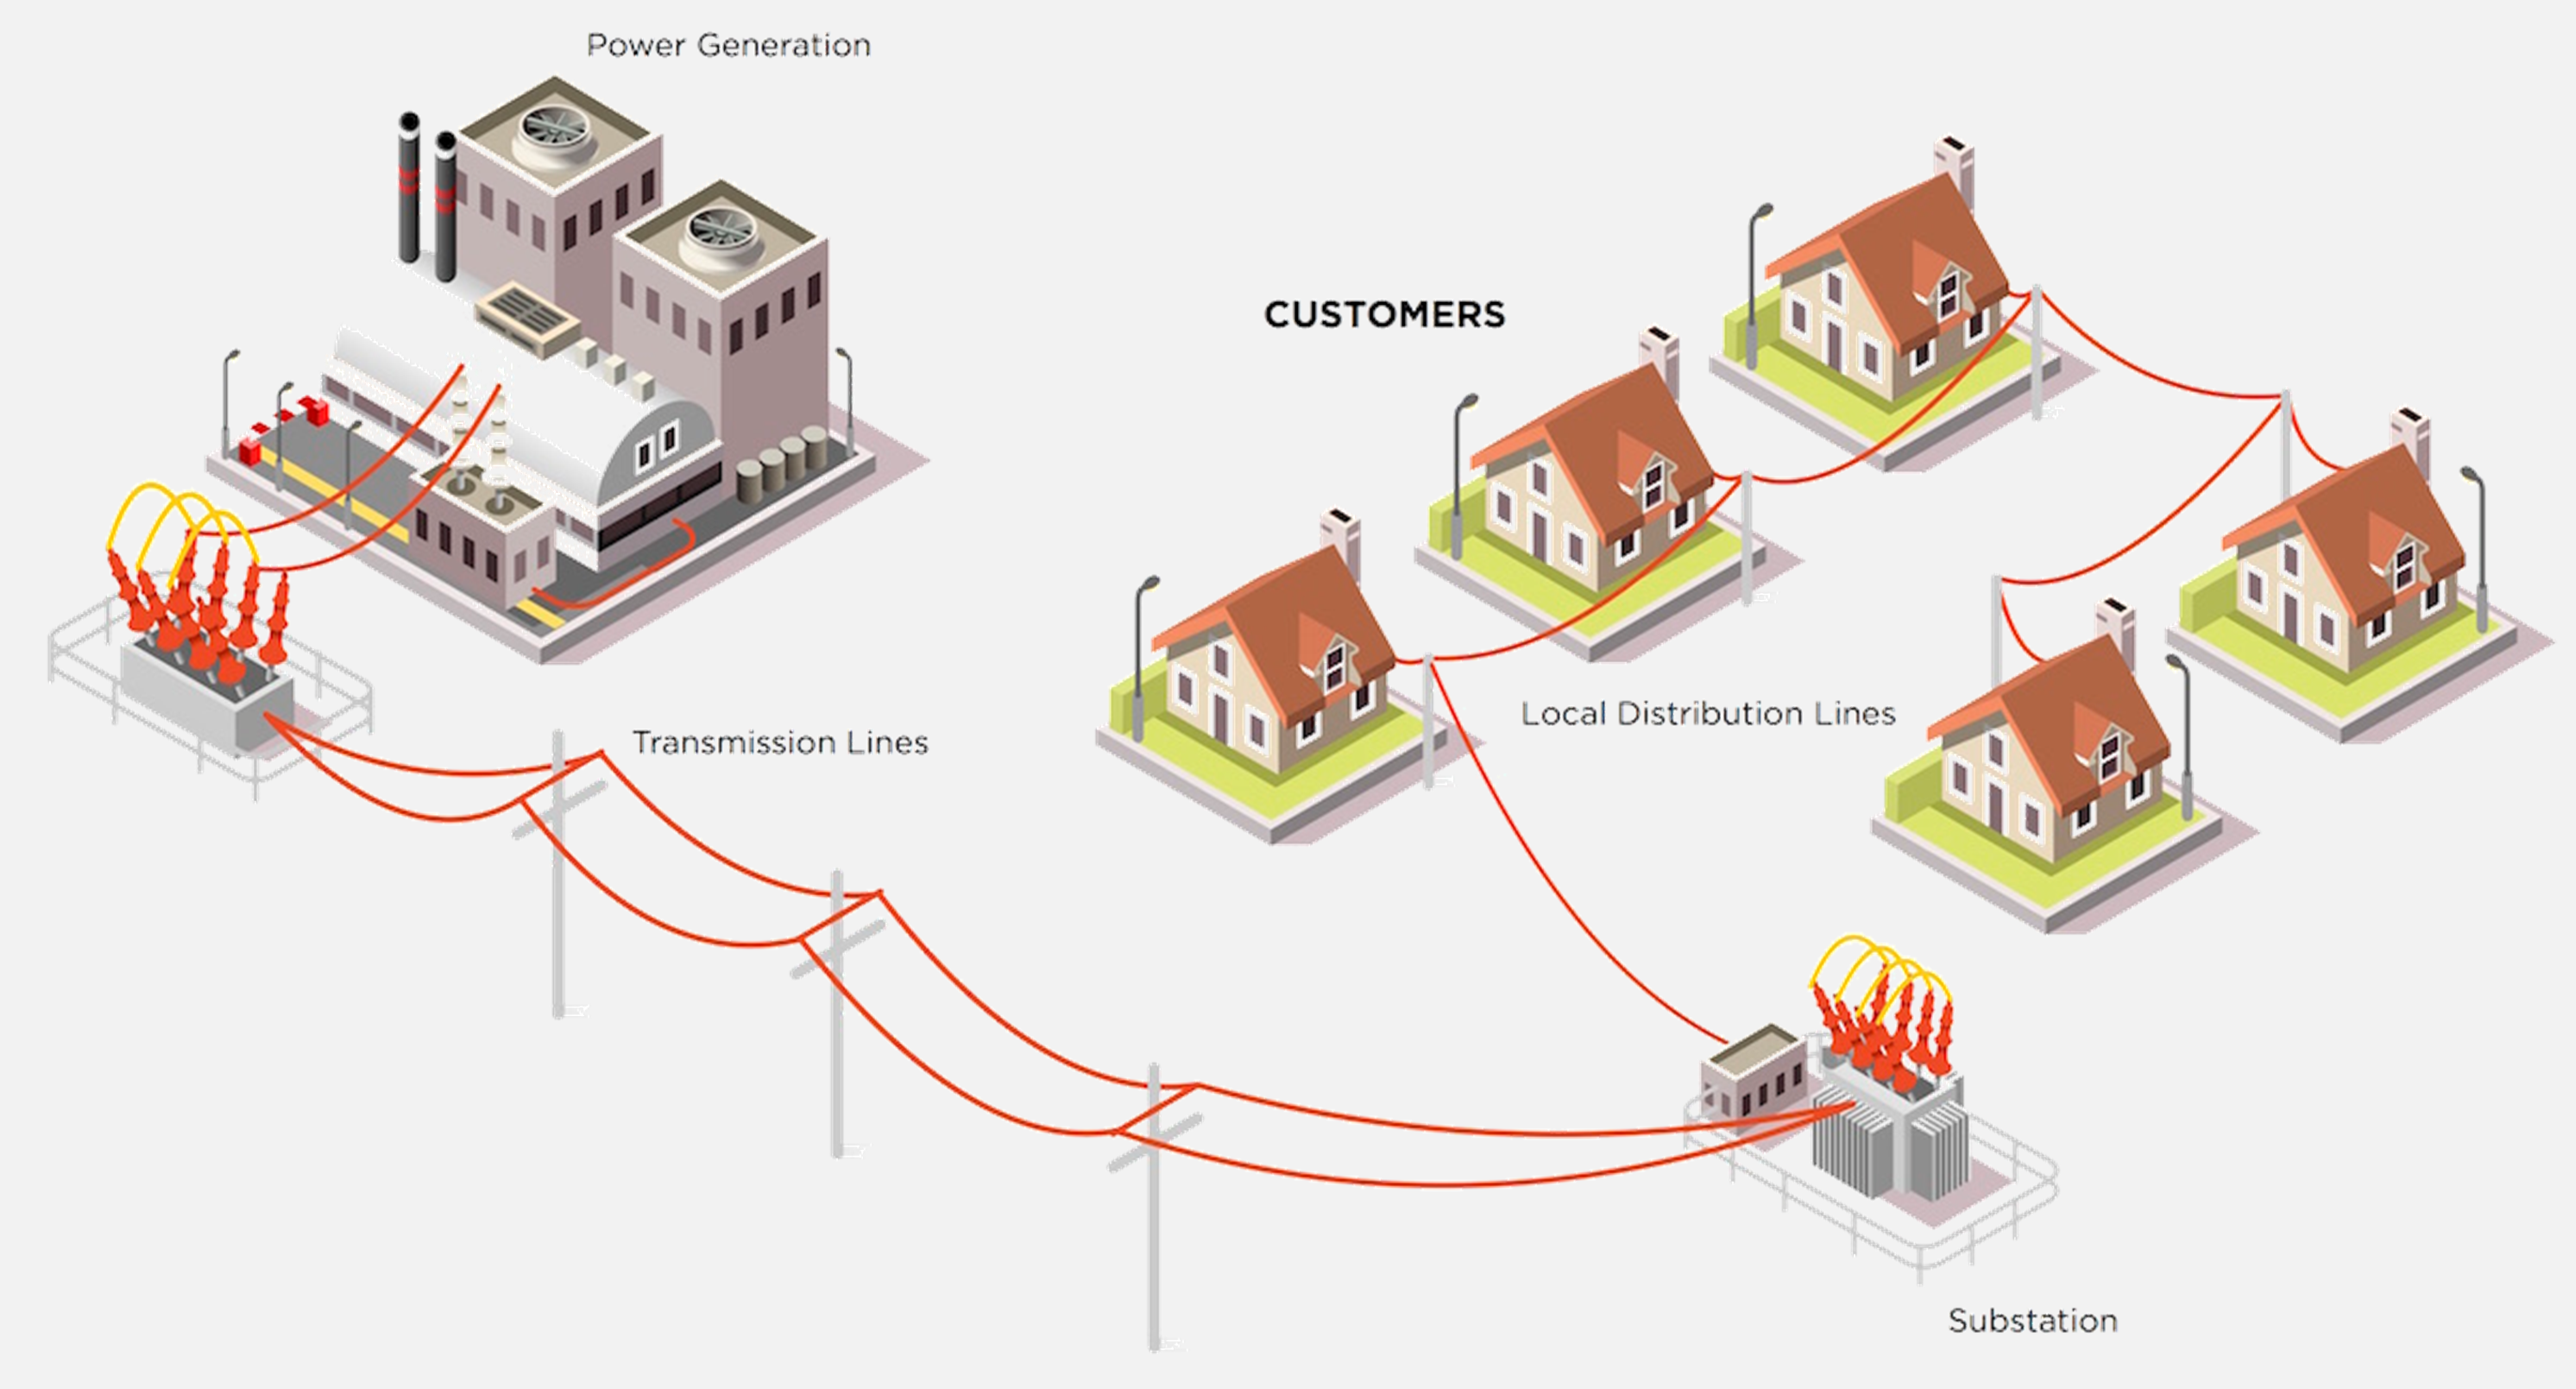
\includegraphics[scale=0.06]{Figures/PowerSys.png}
 \caption{A Typical Power System \textcolor{gray}{\tiny[Rochester Gas \& Electricity]}}
\end{figure}

\end{frame}
	%%%%%%%%%%%%%%%%%%%%%%%%%%%%%%%%%
%%%%%%%%%%%%%%%%%%%%%%%%%%%%%%%%%%%
%%%%%%%%%%%%%%%%%%%%%%%%%%%%%%%%%%%%
%%%%%%%%%%%%%%%%%%%%%%%%%%%%%%%%%%%
%%%%%%%%%%%%%%%%%%%%%%%%%%%%%%%%%
\begin{frame}{Challenges in the planning and operation of the grid}
\begin{itemize}
\item<1-> \textbf{Planning:} Optimizing the right type, size and timing of new grid investments
\begin{itemize}
\item Local generation (e.g. PV) and increased load (e.g. EVs)  can be located in areas where the grid is weak
\item Energy storage and demand flexibility are alternatives to grid reinforcements
\end{itemize}

\item<2-> \textbf{Operation:}Optimize the use of controllable assets such as energy storage and flexible demand to secure, reliable and economic operation of the distribution grids. This means:
\begin{itemize}
\item Making the right use of Demand Response
\item being able to value the use of end-user flexibility for local or system-wide grid services
\item Simulating and optimizing the grids in the presence of \textbf{future local markets for energy and flexibility}
\end{itemize}
\end{itemize}
\end{frame}
%%%%%%%%%%%%%%%%%%%%%%%%%%%%%%%%%
%%%%%%%%%%%%%%%%%%%%%%%%%%%%%%%%%%%
%%%%%%%%%%%%%%%%%%%%%%%%%%%%%%%%%%%%
%%%%%%%%%%%%%%%%%%%%%%%%%%%%%%%%%%%
%%%%%%%%%%%%%%%%%%%%%%%%%%%%%%%%%
\begin{frame}{Limitations of traditional grid operation and planning}
\vskip -1cm
\begin{block}{Notes}
{\scriptsize 
\begin{itemize}
\item<1-> Classical single-period OPF does not offer a possibility for optimal operational scheduling of storage and flexible demand
\item<2->  We therefore aim to develop the foundations for a new generation of Multi-Period OPF (MPOPF) solvers 
\begin{enumerate}[i.]
{\tiny
\item Solves the OPF problem over several coupled time-steps
\item Computation time is an issue when using both commercial or free optimization solvers
}
\end{enumerate}
\item<3-> MPOPF is an extremely challenging scientific task:
\begin{enumerate}[i.]
{\tiny
\item Nonlinearity
\item Large-scale problem with respect with to time and space
\item Involves stochastic generations and load}
\end{enumerate}
\end{itemize}}
\onslide<4>{\begin{alertblock}{Hardware is reaching its limit with respect to CPU clock speed}
\end{alertblock}}
\end{block}
\begin{backgroundblock}{10mm}{50mm}
 \begin{tikzpicture}
    \node[anchor=east,inner sep=0] (B) at (4,0) {
\includegraphics[scale=0.8]{Figures/CPUSpeed.jpg}};
           \fill [draw=none, fill=white, fill opacity=0.5] (B.north west) -- (B.north east) -- (B.south east) -- (B.south west) -- (B.north west) -- cycle;
    \end{tikzpicture} 
   \end{backgroundblock}
\end{frame}
	%%%%%%%%%%%%%%%%%%%%%%%%%%%%%%%%%
%%%%%%%%%%%%%%%%%%%%%%%%%%%%%%%%%%%
%%%%%%%%%%%%%%%%%%%%%%%%%%%%%%%%%%%%
%%%%%%%%%%%%%%%%%%%%%%%%%%%%%%%%%%%
%%%%%%%%%%%%%%%%%%%%%%%%%%%%%%%%%
\begin{frame}{Solution:}
\begin{block}{High-Performance Solver [1-2]}
\begin{itemize}
\item<1-> Algorithmic design tailored to the conventional OPF algorithms speed-up the solution proposal
\item<1-> Prototype model shows convincing results for real-sized system with distributed renewables, storages and EVs

\begin{enumerate}[i.]
{\tiny
\item A high-performance and memory-efficient sparse algorithm 
\item Utilizing the structure of the underlying mathematical formulation}
\end{enumerate}
\end{itemize}
\end{block}

\onslide<2->{\begin{block}{Benefits}
\begin{itemize}
\item<2-> Optimal utilization of \textbf{stored energy} and \textbf{flexibility} where and when it creates the highest value for the system
\item<3-> Can be used for grid planning, grid operation and local markets
\end{itemize}
\end{block}}
\begin{enumerate}
{\tiny 
\item S. Zaferanlouei, H. Farahmand, V. V. Vadlamudi, M. Korpås,“BATTPOWER Toolbox: Memory-Efficient and High-Performance Multi-Period AC Optimal Power Flow Solver”, IEEE Transactions on Power Systems, Jan. 16th, 2021.
\item S. Zaferanlouei, et al., “BATTPOWER Application: Large-Scale Integration of EVs in an Active Distribution Grid ---A Norwegian Case Study”, Under review in the journal of EPSR}
 \end{enumerate}
\end{frame}
%%%%%%%%%%%%%%%%%%%%%%%%%%%%%%%%%%%%%%%%%
%%%%%%%%%%%%%%%%%%%%%%%%%%%%%%%%%%%%%%%%%
%%%%%%%%%%%%%%%%%%%%%%%%%%%%%%%%%%%%%%%%%
%%%%%%%%%%%%%%%%%%%%%%%%%%%%%%%%%%%%%%%%%
\begin{frame}{Power System--- Today}
\centering
\animategraphics[loop,width=10cm]{12}{Figures/gif/Today/01-}{0}{115}
{\tiny[Reference: Joint Research Centre: Eurpean Commission Web page\\
https://ses.jrc.ec.europa.eu/smart-grid-interactive-tool-non-flash]}
\end{frame}
%%%%%%%%%%%%%%%%%%%%%%%%%%%%%%%%%%%%%%%%%%
%%%%%%%%%%%%%%%%%%%%%%%%%%%%%%%%%%%%%%%%%%
%%%%%%%%%%%%%%%%%%%%%%%%%%%%%%%%%%%%%%%%%%
%%%%%%%%%%%%%%%%%%%%%%%%%%%%%%%%%%%%%%%%%%
\begin{frame}{Power System--- Future}
\centering
\animategraphics[loop,width=10cm]{12}{Figures/gif/Future/01-}{0}{98}
{\tiny[Reference: Joint Reseach Centre: Eurpean Commission Web page\\
https://ses.jrc.ec.europa.eu/smart-grid-interactive-tool-non-flash]}
\end{frame}


%%%%%%%%%%%%%%%%%%%%%%%%%%%%%%%%%%%%%%%%%%
%%%%%%%%%%%%%%%%%%%%%%%%%%%%%%%%%%%%%%%%%%
%%%%%%%%%%%%%%%%%%%%%%%%%%%%%%%%%%%%%%%%%%
%%%%%%%%%%%%%%%%%%%%%%%%%%%%%%%%%%%%%%%%%%


\begin{frame}[plain]
\begin{tikzpicture}[overlay, remember picture]
\node[anchor=center] at (current page.center) {
\begin{beamercolorbox}[center]{title}
     Phase II:\\\textbf{EV Statistics}
  \end{beamercolorbox}};
\end{tikzpicture}

\end{frame}



%%%%%%%%%%%%%%%%%%%%%%%%%%%%%%%%%
%%%%%%%%%%%%%%%%%%%%%%%%%%%%%%%%%%%
%%%%%%%%%%%%%%%%%%%%%%%%%%%%%%%%%%%%
%%%%%%%%%%%%%%%%%%%%%%%%%%%%%%%%%%%
%%%%%%%%%%%%%%%%%%%%%%%%%%%%%%%%%

\begin{frame}{Statistics}
\only<1>{
\begin{block}{Market Share}
Market share of electric cars (BEV and PHEV) in Norway from 2009 to 2019[ssb.no]
\end{block}
\center
        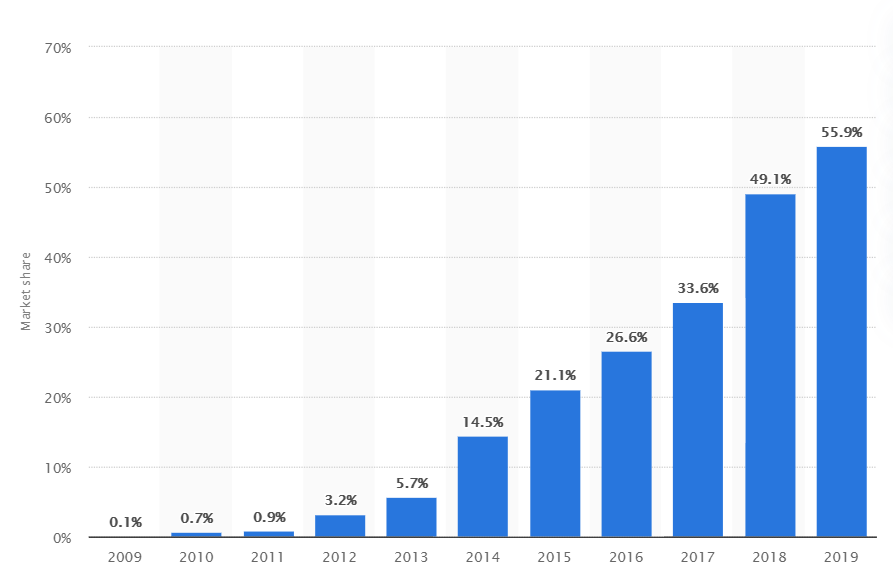
\includegraphics[scale=0.4]{Figures/marketShare.png}}
        \only<2>{
\begin{alertblock}{Penetration}
Around 10\% EV penetration in Norwegian transport sector. The Norwegian Parliament has decided on a national goal that all new cars sold by 2025 should be zero-emission (electric or hydrogen)\footnote{https://elbil.no/}.
\end{alertblock}}
\end{frame}

%%%%%%%%%%%%%%%%%%%%%%%%%%%%%%%%%%%%%%%%%%
%%%%%%%%%%%%%%%%%%%%%%%%%%%%%%%%%%%%%%%%%%
%%%%%%%%%%%%%%%%%%%%%%%%%%%%%%%%%%%%%%%%%%
%%%%%%%%%%%%%%%%%%%%%%%%%%%%%%%%%%%%%%%%%%%
%\section{Motivation}	
%\begin{frame}{Motivation}
%		\begin{enumerate}
%  			\item<1-> \vskip -1cm Sustainability: {\footnotesize Need tools for analysing operating conditions resulting from renewables, EV, storage and flexible demand.}
%  			\only<1>{\begin{backgroundblock}{40mm}{30mm}
%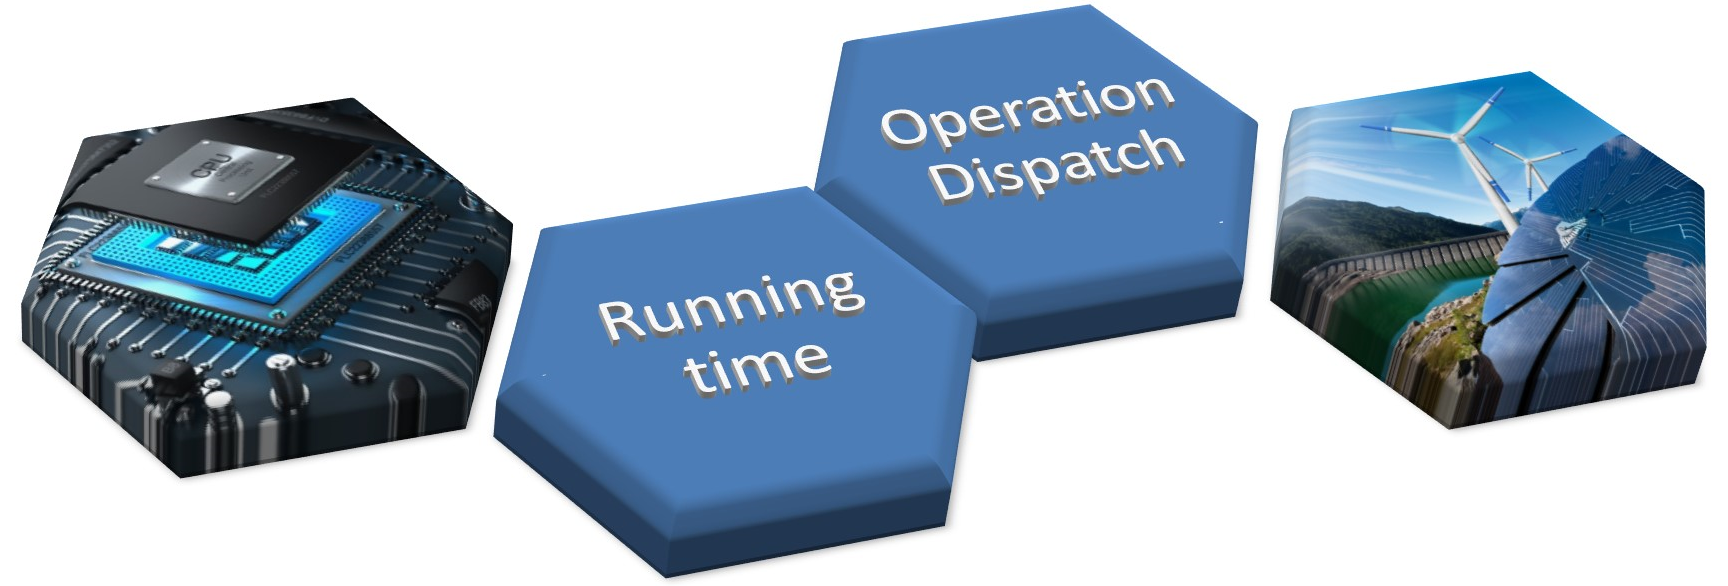
\includegraphics[width=100mm]{Figures/pageMotive.png}
%\end{backgroundblock}}
%			\item<2-> Economics: {\footnotesize Norway electric industry revenues of 61.6 billion NOK in 2018\footnote{\label{note1} \tiny https://www.nve.no/energy-market-and-regulation/retail-market/electricity-disclosure-2018/}. 1\% savings worth 615 million NOK (estimated using \textsuperscript{\ref{note1}} \textsuperscript{and} \footnote{\tiny{https://www.nordpoolgroup.com/Market-data1/Dayahead/Volumes/NO/Hourly/?view=table}})} 
%
%			\item<3-> Reliability: {\footnotesize Annual cost of power interruptions to Norway economy is 1600 MNOK/year (estimated using \footnote{\tiny http://publikasjoner.nve.no/rapport/2018/rapport2018\_74.pdf} \textsuperscript{and} \footnote{\tiny Samdal, K., Kjolle, G. H., Singh, B., \& Kvitastein, O. (2006, June). Interruption costs and consumer valuation of reliability of service in a liberalised power market. In 2006 International Conference on Probabilistic Methods Applied to Power Systems (pp. 1-7). IEEE.})   }
%	\end{enumerate}
%		\end{frame}	
%%%%%%%%%%%%%%%%%%%%%%%%%%%%%%%%%%%%%%%%%%
%%%%%%%%%%%%%%%%%%%%%%%%%%%%%%%%%%%%%%%%%%
%%%%%%%%%%%%%%%%%%%%%%%%%%%%%%%%%%%%%%%%%%
%%%%%%%%%%%%%%%%%%%%%%%%%%%%%%%%%%%%%%%%%%
\begin{frame}[plain]
\begin{tikzpicture}[overlay, remember picture]
\node[anchor=center] at (current page.center) {
\begin{beamercolorbox}[center]{title}
     Phase III:\\\textbf{Case Study}
  \end{beamercolorbox}};
\end{tikzpicture}

\end{frame}

%	%%%%%%%%%%%%%%%%%%%%%%%%%%%%%%%%%
%%%%%%%%%%%%%%%%%%%%%%%%%%%%%%%%%%%%
%%%%%%%%%%%%%%%%%%%%%%%%%%%%%%%%%%%%%
%%%%%%%%%%%%%%%%%%%%%%%%%%%%%%%%%%%%
\begin{frame}{Steinkjer Demo: a Real Distribution Grid}
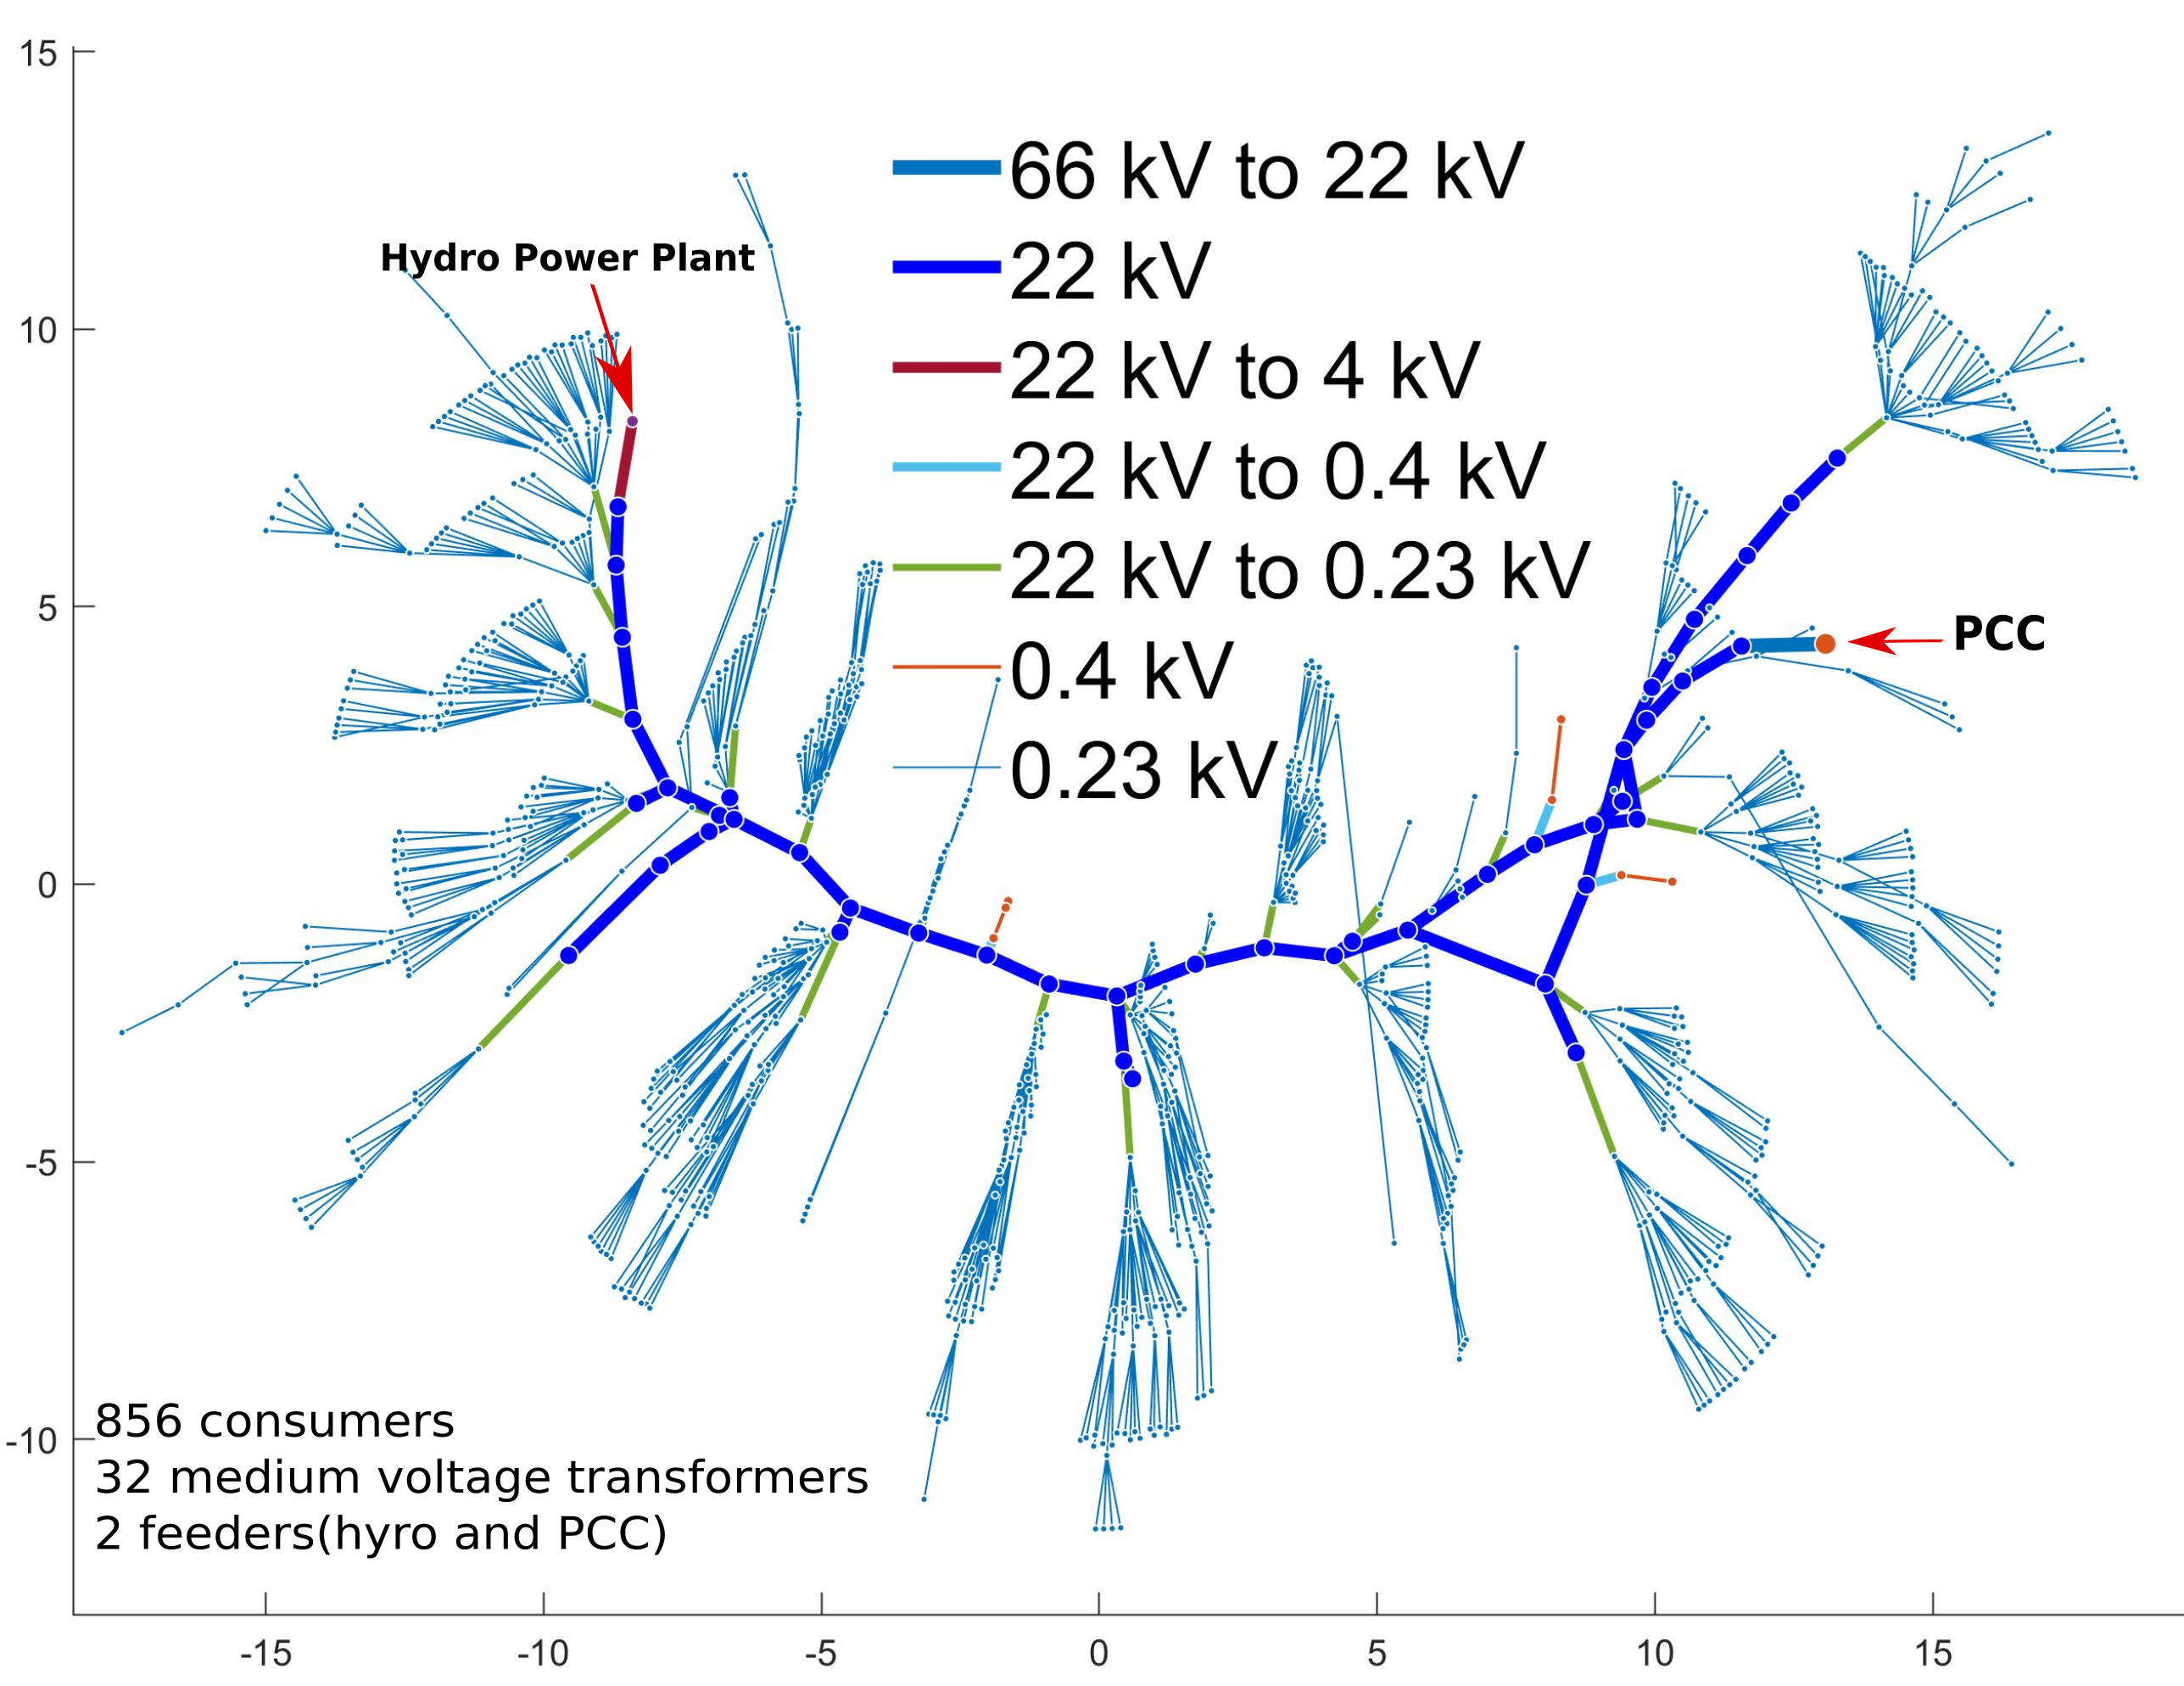
\includegraphics[width=100mm, height=70mm]{Figures/DistributionGrid26082021.png}


\end{frame}
%%%%%%%%%%%%%%%%%%%%%%%%%%%%%%%%%%%%%%%%%%
%%%%%%%%%%%%%%%%%%%%%%%%%%%%%%%%%%%%%%%%%%
%%%%%%%%%%%%%%%%%%%%%%%%%%%%%%%%%%%%%%%%%%
%%%%%%%%%%%%%%%%%%%%%%%%%%%%%%%%%%%%%%%%%%
\begin{frame}{Simulations through time}
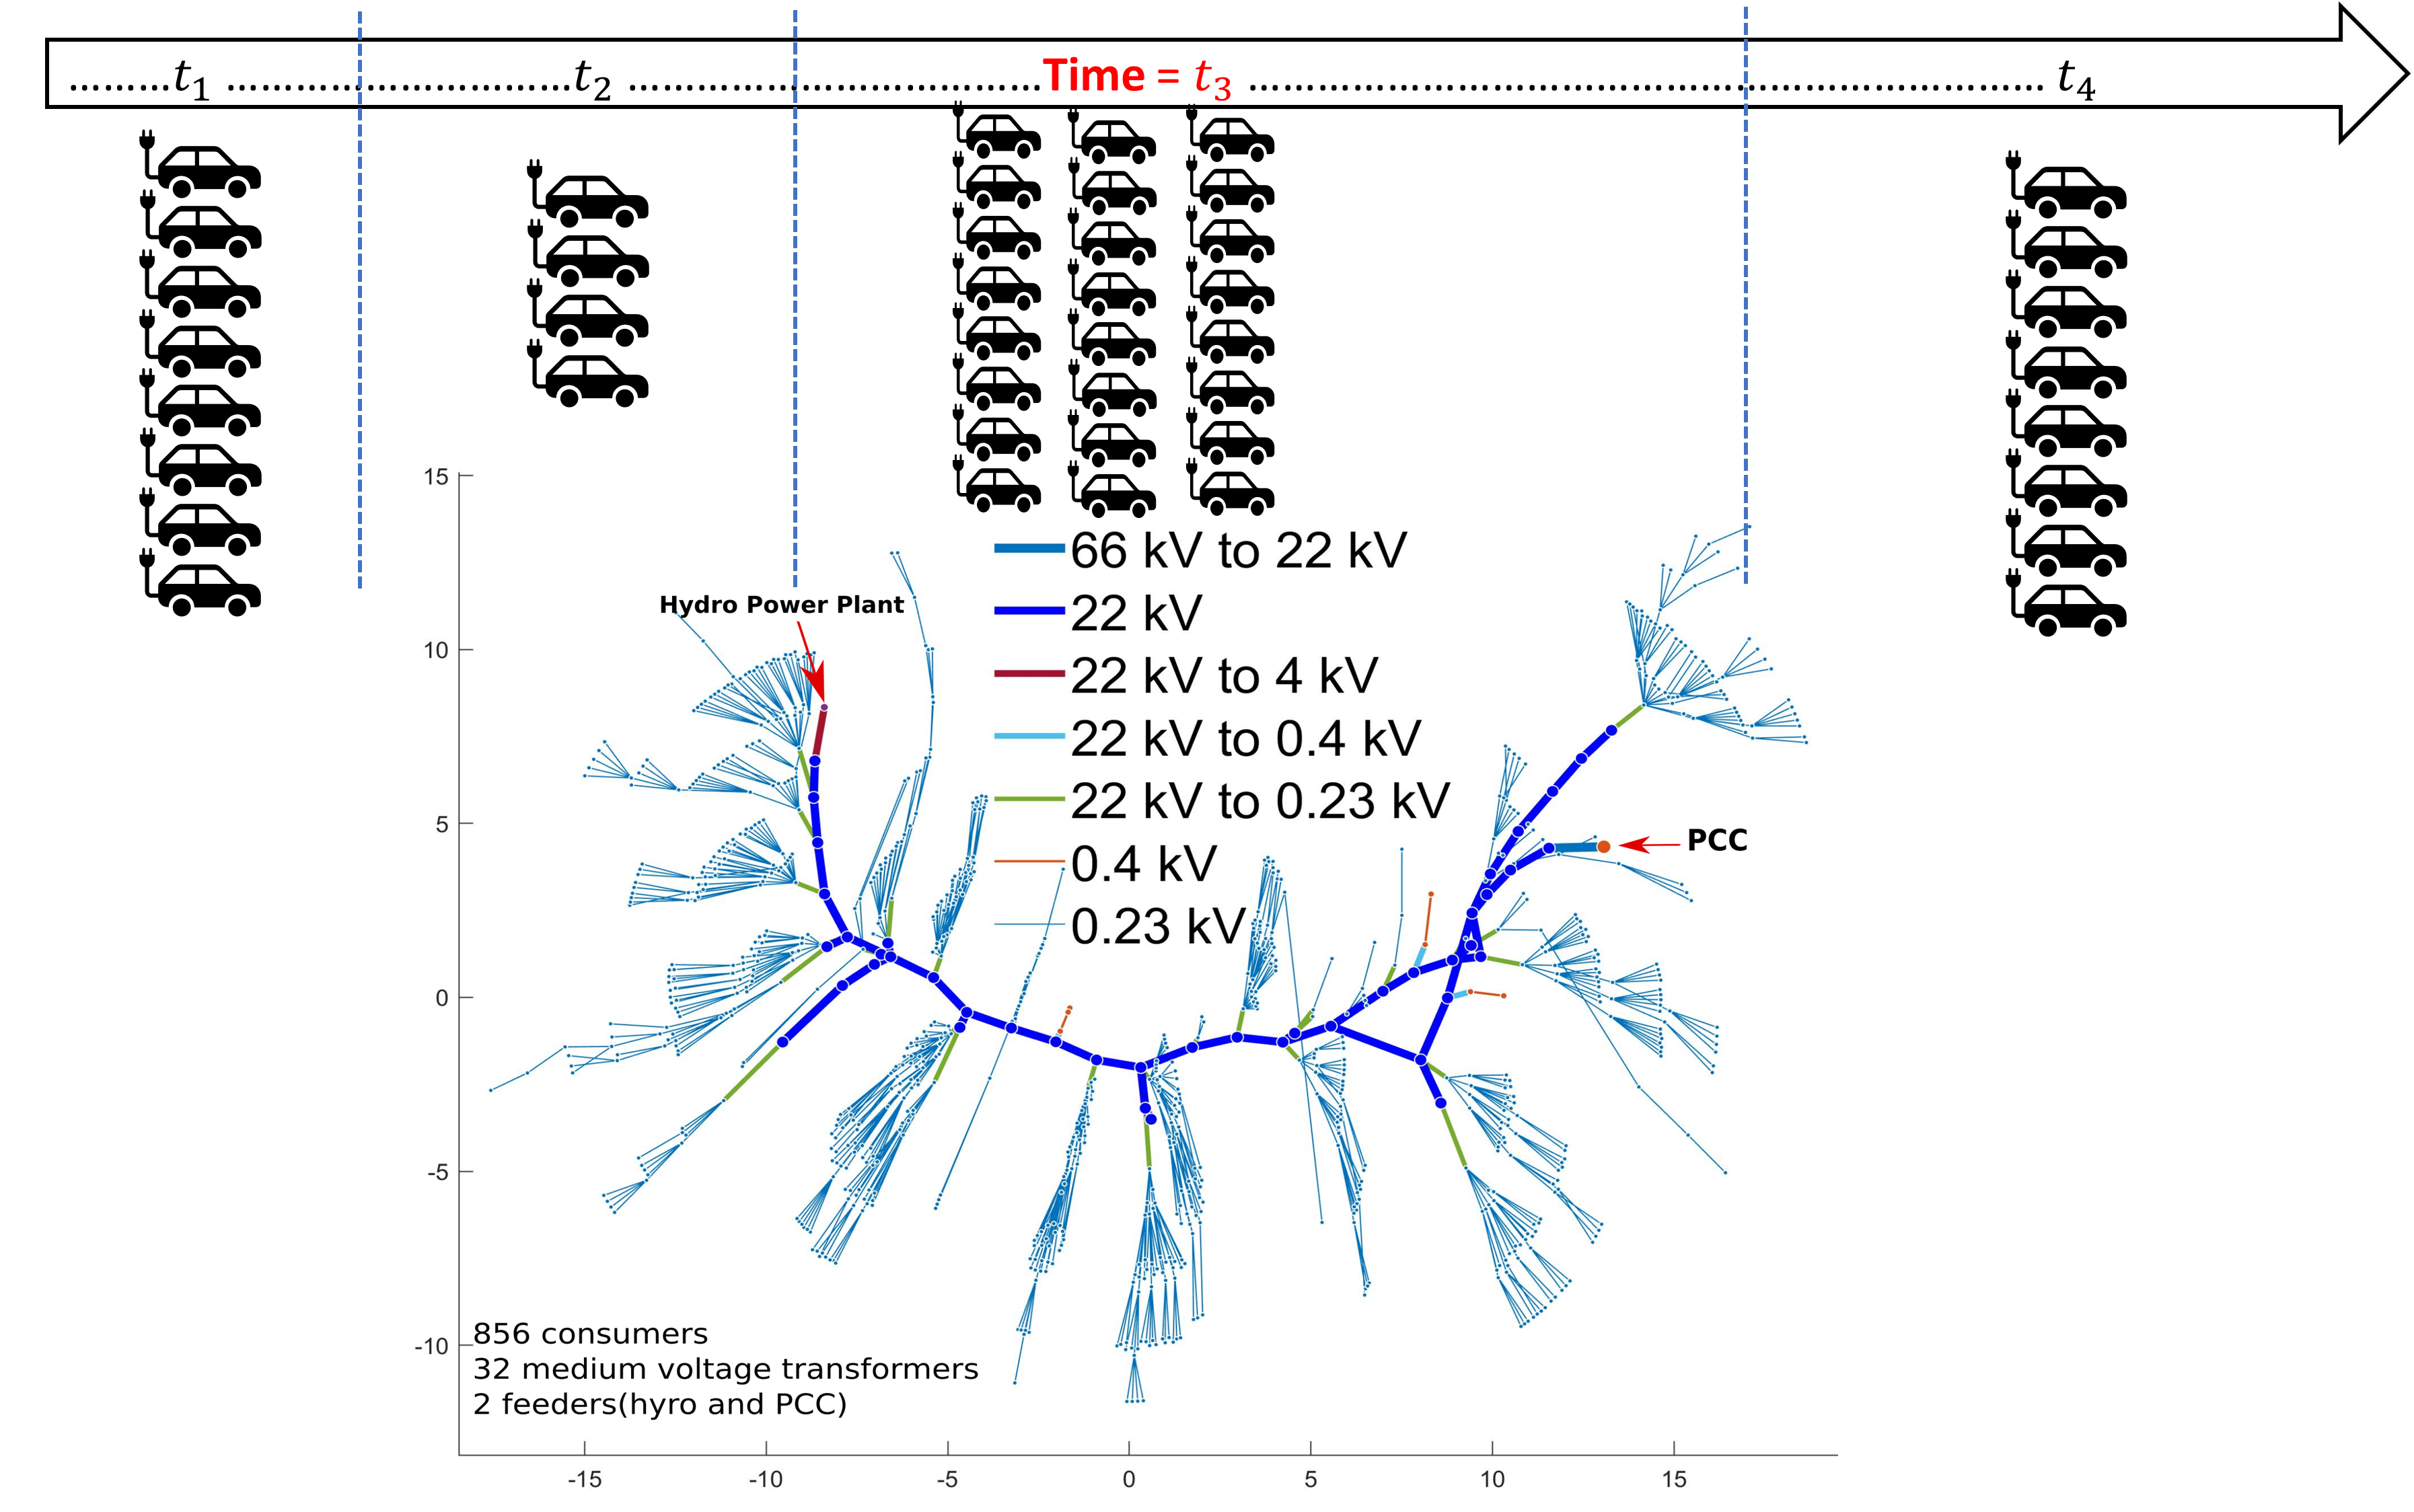
\includegraphics[width=110mm, height=70mm]{Figures/CaseStudy/CaseStudy.png}
\end{frame}

%%%%%%%%%%%%%%%%%%%%%%%%%%%%%%%%%%%%%%%%%%
%%%%%%%%%%%%%%%%%%%%%%%%%%%%%%%%%%%%%%%%%%
%%%%%%%%%%%%%%%%%%%%%%%%%%%%%%%%%%%%%%%%%%
%%%%%%%%%%%%%%%%%%%%%%%%%%%%%%%%%%%%%%%%%%

\begin{frame}{Simulation Results}
{\tiny
\begin{table}
\def\firstrowcolor{}
\def\secondrowcolor{}
\onslide<1->{\def\firstrowcolor{\rowcolor{Gray}}}
\caption{Charge Scheduling Strategies}
\label{tab:termination}
\begin{tabular}{l l c c} 
\hline
 \firstrowcolor Method & Description &\begin{tabular}[c]{@{}c@{}}Max EV\\ hosting Capacity\end{tabular}&  \\  
  Uncoordinated/Dumb Charging&Charge on arrival time& 20\%& 
\includegraphics[width=.1\textwidth]{Figures/RedMark.png} \\
 \onslide<2->{Market price based &\only<2>{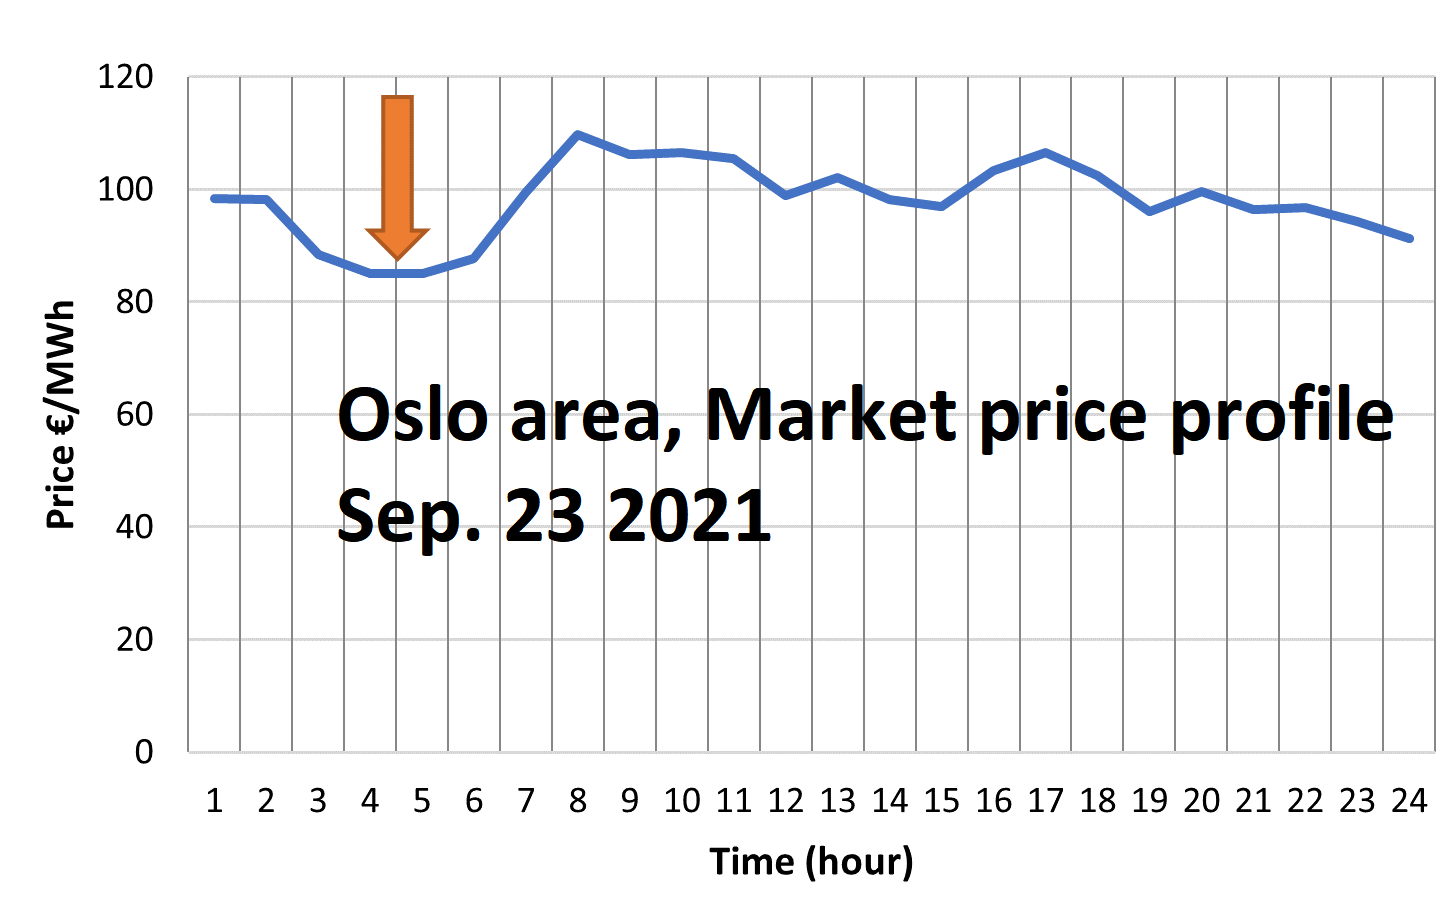
\includegraphics[width=40mm, height=30mm]{Figures/CaseStudy/OsloPrice.png}}
 & 36\%& 
\includegraphics[width=.1\textwidth]{Figures/YellowMark.png}} \\
 \onslide<3->{\begin{tabular}[c]{@{}l@{}}Market price and\\ Congestion management based\end{tabular}& \only<3>{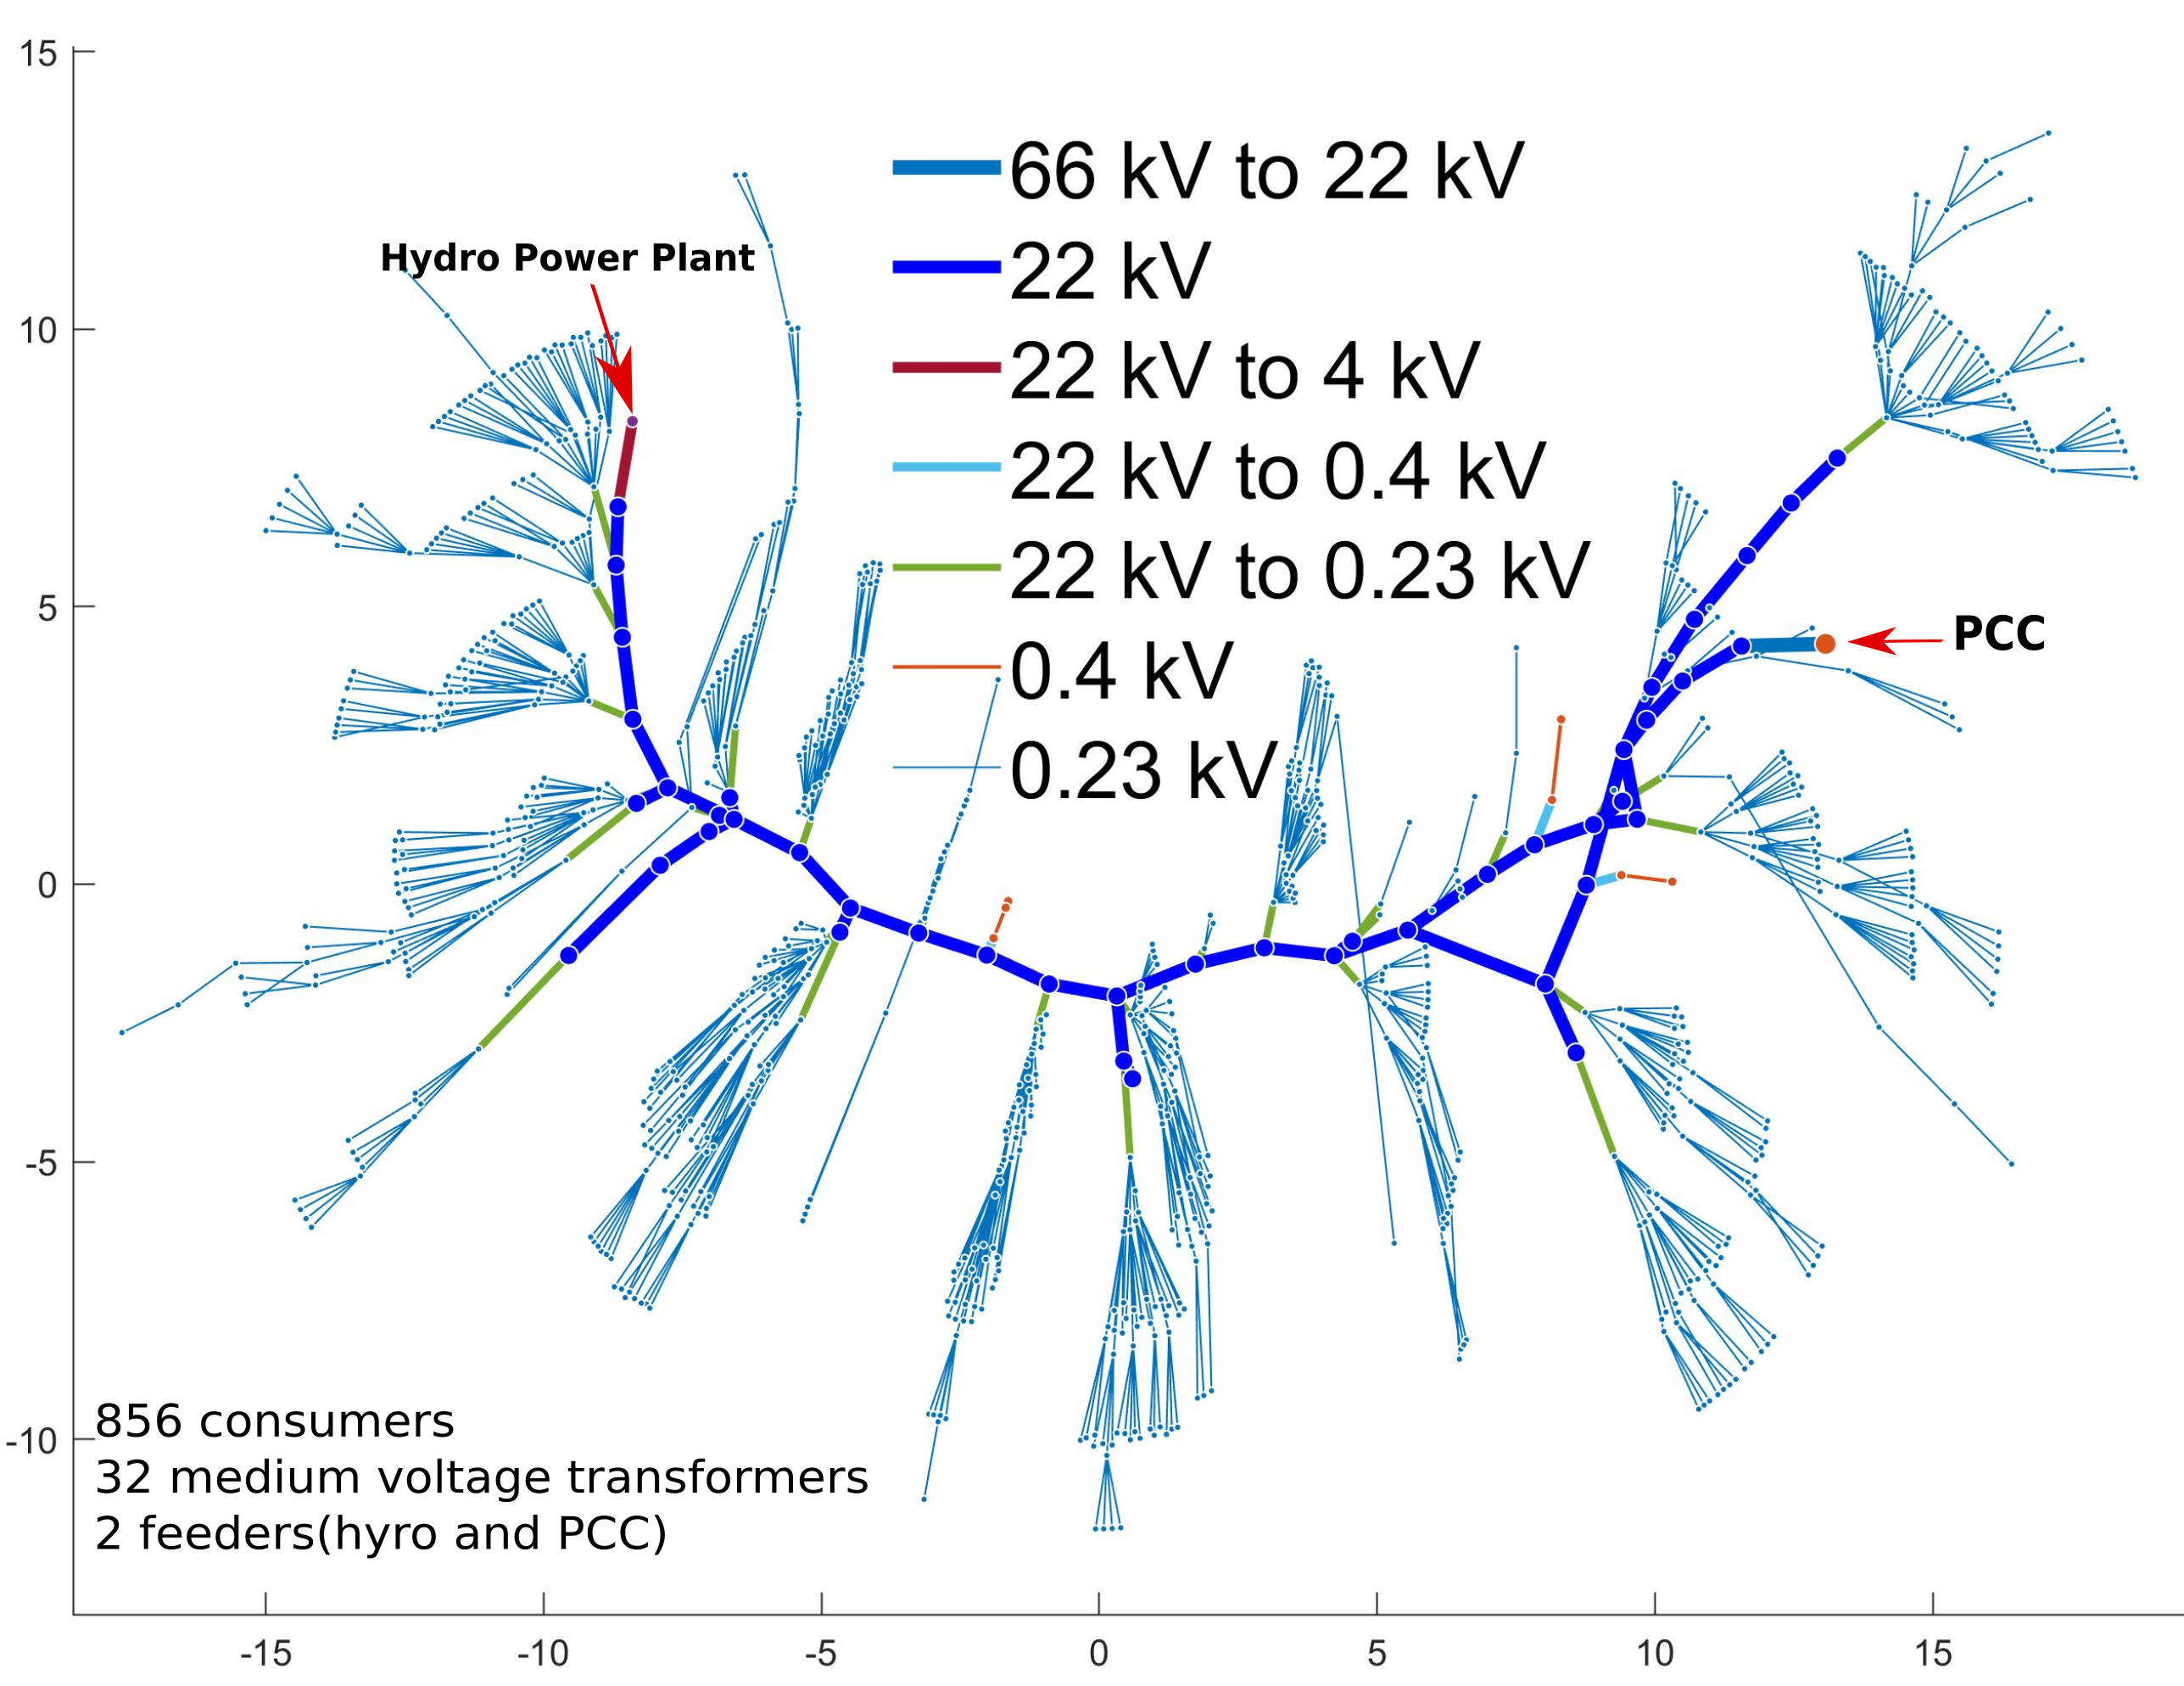
\includegraphics[width=40mm, height=30mm]{Figures/DistributionGrid26082021.png}}&100\%& 
\includegraphics[width=.1\textwidth]{Figures/GreenMark.png} }\\
\hline
\end{tabular}
\end{table}
}

\end{frame}
%	%%%%%%%%%%%%%%%%%%%%%%%%%%%%%%%%%
%%%%%%%%%%%%%%%%%%%%%%%%%%%%%%%%%%%%
%%%%%%%%%%%%%%%%%%%%%%%%%%%%%%%%%%%%%
%%%%%%%%%%%%%%%%%%%%%%%%%%%%%%%%%%%%

%\begin{frame}{Summary}
%\begin{block}{Highlights}
%{\scriptsize
%\begin{itemize}
%\item<1-> 
%\item<2-> 
%\item<3-> 
%\item<4-> 
%\end{itemize}
%}
%\end{block}
%\end{frame}

%%%%%%%%%%%%%%%%%%%%%%%%%%%%%%%%%%%%%%%%%%%
%%%%%%%%%%%%%%%%%%%%%%%%%%%%%%%%%%%%%%%%%%%
%%%%%%%%%%%%%%%%%%%%%%%%%%%%%%%%%%%%%%%%%%%
%%%%%%%%%%%%%%%%%%%%%%%%%%%%%%%%%%%%%%%%%%%
%\begin{frame}{Power System--- Future}
%\centering
%\animategraphics[loop,width=10cm]{12}{Figures/gif/Future/01-}{0}{98}
%\end{frame}


\begin{frame}
\centering
Thank you for your attention!\\
		\vskip 0.8cm

\centering

\includegraphics[scale=0.2]{ntnulogo_eng.png}
\end{frame} 

\end{document}


